% !TEX root = ../../main.tex



\chapter{Experimental Evaluation} \label{chap:evaluation}

\minitoc

We evaluate the performance of CALock and experimentally compare it with the state of the art. Our evaluation uses the same benchmarks as DomLock, MID and FlexiGran \cite{kalikar2016domlock,anjuMID,FlexiGran2024} i.e. STMBench7\cite{guerraoui2006stmbench7}. In this chapter, we first present the experimental setup and then the results of the experiments and discuss their implications. 

We run our experiments on a machine with an AMD EPYC 7642 CPU, with 48 Cores, a base clock of 2.3 GHz and 512 GB of RAM \footnote{Experiments presented in this thesis were carried out using the Grid'5000 testbed, supported by a scientific interest group hosted by Inria and including CNRS, RENATER and several Universities as well as other organizations (see https://www.grid5000.fr).}. 
The benchmark is deployed on a Docker container under Ubuntu 20.04. 
To build the benchmark, GCC 12.1 and Cmake 3.22 are used. The compilation is done at the C++ 23 standard to enable the use of atomic wait primitives. The optimization level is set to O3.




\section{Benchmark Suite: STMBench7}
	
	
	\begin{figure}
		\centering
		\captionsetup{justification=centering}
		\includegraphics[width=.8\columnwidth]{figures/stmbenchModule}
		\caption{Structure of a module in STMBench with medium lock boundaries}
		\label{stmbenchModule}
	\end{figure}

	% \begin{table}[ht]
	% 	\begin{tabular}{l*{5}{l}}
	% 		Size & Vertices & {Complex Assemblies} & Base Assemblies & Composite parts & Atomic Parts \\ \hline
	% 		Small  & 1000   & 111  	& 132 	& 167 	& 16700		\\ \hline
	% 		Medium & 10000  & 132 	& 206 	& 534 	& 53255 		\\ \hline
	% 		Large  & 100000 & 96 	& 118	& 269 	&  134500	\\ \hline
	% 	\end{tabular}
	% \end{table}
STMBench is a well known benchmark based on the classical OO7 object oriented benchmark suite \cite{CareyDN93}. It is widely used to evaluate the performance of hierarchical algorithms and data structures \cite{prokopec_renaissance_2019,vale_pot_2016, felber_hardware_2016, carvalho_optimizing_2016, kim_scheduling_2015,filipe_nested_2015,rito_props_2014,kalikar2016domlock,anjuMID,FlexiGran2024,KalikarN18,GaneshKN18,liu_unleashing_2014} 

The hierarchy in STMBench7, as represented in Figure \ref{stmbenchModule}, consists of a \emph{module} at the root level. This module consists of several levels of \emph{complex assemblies}. 
Each of the deepest complex assemblies consists of a set of \emph{base assemblies}. 
A \emph{composite part} can be contained in several base assemblies. 
Each composite part contains a set of \emph{atomic parts}. 
These atomic parts form a near-complete graph. 
The root of this graph is connected to a single composite part.

STMBench7 provides coarse-grain  and medium-grain lock implementations. These are representatives of fixed granularity locking techniques, used in practice.  
The coarse-grain lock is a reader-writer lock on the entire graph. 
Figure  \ref{stmbenchModule} shows the medium-grain lock grains for a module. 
Complex assemblies are divided into levels and each level is guarded by its own lock.
Deeper in the graph, the set of atomic parts, under each composite part, is guarded by its own lock.
A structural modification operation acquires a mutex on the entire graph.


STMBench provides a set of operations that stress the locking mechanism being evaluated. From these operations, Q1 and Q2 are read-only operations, OP1 and OP2 are read-write operations and SM1 and SM2 are structural modification operations.
\begin{enumerate}
	\item Reading an atomic part (Q1).
	\item Reading a set of atomic parts (Q2).
	\item Reading a complex assembly (OP1).
	\item Reading a set of complex assemblies (OP1).
	\item Reading a base assembly (OP2).
	\item Reading a set of base assemblies (OP2).
	\item Writing data to an atomic part (OP3).
	\item Writing data to a set of atomic parts (OP4).
	\item Deleting a composite part (SM1).
	\item Adding an edge between a base assembly and a composite part (SM2).
\end{enumerate}
	%These operations together form a load consisting of queries that lead to multiple lock granularities and stress the lock acquisition as well as conflict detection mechanisms. These queries were executed with varying proportions of reads and writes on both, static and dynamic hierarchies. Several benchmark parameters were collected.
	% The provided implementation of DomLock uses busy-waiting. For a more fair comparison, we modified DomLock to use a condition variable, as CALock does.

% \subsection{Stress benchmark} 
% In addition to STMBench, we provide a synthetic stress benchmark that uses a balanced static binary tree with 1 million vertices. 
% Each vertex in this tree has an ID and pointers to its children and its parent. 
% The tree does not change during the runtime of the benchmark.  
% A thread selects one or more leaf nodes in the tree to lock. 
% To stress contention, the benchmark always takes a write lock since two write lock requests conflict when their grains overlap. 

% In the stress benchmark, we compare \emph{Intention locks, DomLock and CALock}. 
% DomLock and CALock store the intervals and labels of the vertices respectively. 
% For intention locks, as an optimization, we pre-compute and store the paths to a vertex to avoid repetitive exploration of the hierarchies to find a vertex. 
% The stress benchmark can be configured to access the specific parts of the tree. 
% For this, the leaves of the tree are organized into buckets. The number of buckets is configurable for a benchmark run.

	\subsection{Synopsis}

	The research questions addressed by our benchmarks compare CALock with DomLock, MID and FlexiGran:

	\begin{description}
		\item[\S \ref{benchmark:PerOpLatency}] How quickly does CALock grant a lock compared to DomLock, MID, FlexiGran for lock requests of different operation types (Q1-SM2)?
		
		\item[\S \ref{benchmark:labellingAndRelabelling}] What is the cost of labelling a hierarchy with CALock labels compared to integer intervals for DomLock, MID and FlexiGran?
		
		\item [\S \ref{benchmark:metadatasize}] How expensive is it to maintain a set of guarding ancestors for each vertex in the hierarchy for CALock compared to integer intervals for DomLock, MID and FlexiGran? 
	
		\item[\S \ref{benchmark:falseSubsumption}] Does CALock eliminate false subsumptions and reduce grain size compared to DomLock, MID and FlexiGran?
		%\item(\S \ref{benchmak:ThreadIdling}) How long does a thread spend waiting for a lock?
		% \item[\S \ref{benchmark:lockRequestSize}] How does the size of a lock request affect the cost of locking?
		% \item[\S \ref{benchmar:lockLocality}] How does lock locality affect performance?
		\item[\S \ref{benchmark:StaticOverallPerf}] What is the performance of CALock compared to other lock strategies for workloads with only data updates (Q1-OP4)?
	
		\item[\S \ref{benchmark:DynamicOverallPerf}] What is the performance of CALock compared to other lock strategies for workloads that also include structual modifications (Q1-SM2)?
	\end{description}
	
	
\section{Per operation response time} \label{benchmark:PerOpLatency}

Figure \ref{ttc} shows the time to completion for different operations in STMBench7. 
% Coarse-grain and medium-grain locks have the fastest response time since they are pthread locks and do not require additional metadata. 
Coarse-grain and Medium-grain locks are the fastest to grant lock requests. However, they do not scale well (see Sections \ref{benchmark:StaticOverallPerf}, \ref{benchmark:DynamicOverallPerf}). 

Intention locks are slower than coarse-grain and medium-grain locks because they require a depth-first traversal to acquire intention locks on the paths that lead to a target vertex. The cost of acquiring intention locks is linear in the number of unique paths to a target vertex. For requests with multiple target vertices (Q2, OP4), this cost is multiplied and leads to a higher response time. 

\begin{figure}[h]
	\captionsetup{justification=centering}
	\centering
	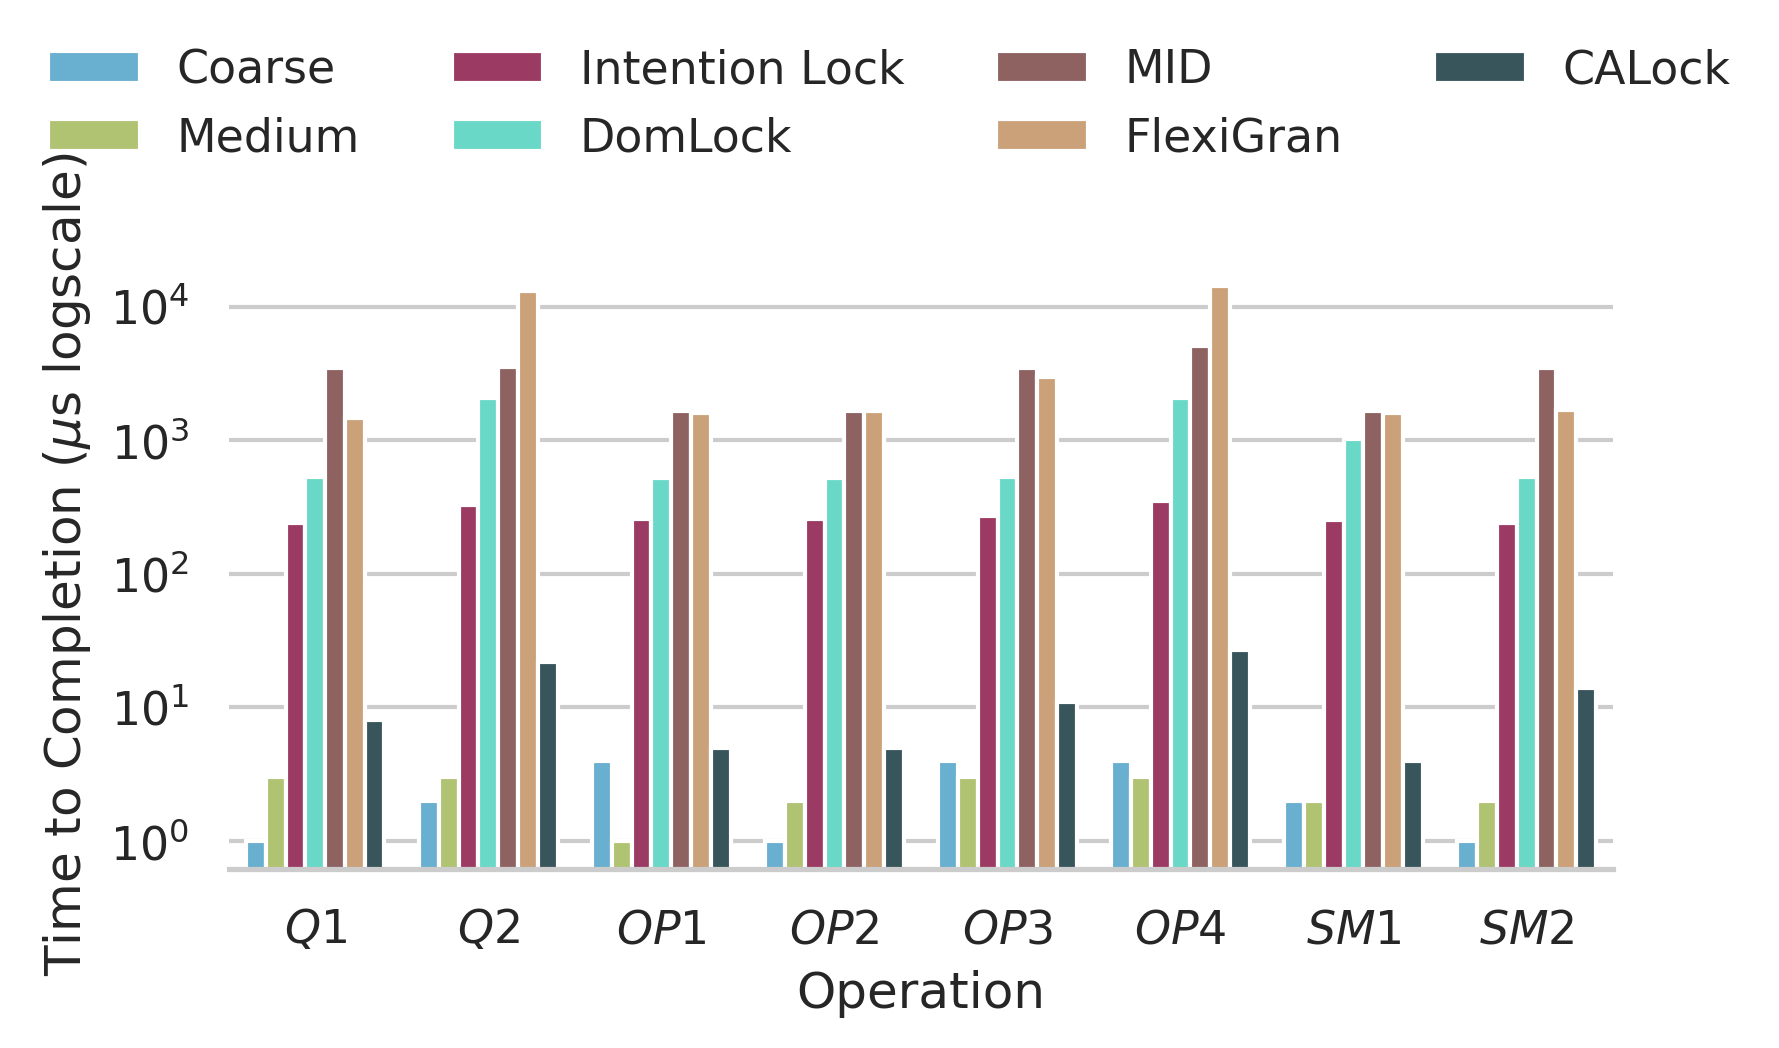
\includegraphics[width=.8\columnwidth]{figures/PerformanceCharts/TTC}
	\caption{Time to completion for different operations in STMBench (lower is better)}
	\label{ttc}
\end{figure}

In MGL techniques like DomLock, MID and FlexiGran, the time to completion is at least $10^{2.5}$ times higher than coarse-grain, medium-grain and intention locks. This is because once a thread identifies the lock targets and finds their interval range, a depth first traversal is required to find the lock guard with the same interval range. This traversal is especially expensive for vertices deeper in the hierarchy.


Between MGL techniques, DomLock is the fastest since conflict detection requires only testing overlap between a pair of intervals. MID is slower than DomLock because it requires testing overlap between two pairs of intervals. FlexiGran is slower than MID because it requires testing overlap between intervals and level numbers. Conflict detection in FlexiGran MGL and FlesiGran fine-grained locks involves testing reachability between the guard of the MGL lock and the fine-grained lock. This is expensive and leads to an overall higher time to completion.

CALock is at least $10^2$ times faster to grant a lock than other MGL techniques. This is because CALock eliminates the need for a traversal to find the lock guard. Instead, a set intersection of the labels is used to find the LGCA which serves as the lock guard. This is significantly faster than the depth-first traversal required by Intention locks, DomLock, MID and FlexiGran.

Read only operations (Q1, Q2) are the fastest since they can progress in parallel, even in the same grain. 
Write operations (OP3, OP4) are slower since they require exclusive access to the grain. Structural modifications often take the longest since they require exclusive access to the entire graph with DomLock, MID and FlexiGran. CALock parallelizes the relabelling of disjoint subgraphs and is at least $10^2$ times faster. 



% For coarse and medium grained locks, reads are fast and finish relatively quickly since they occur under pthread read locks which do not require additional metadata. Write operations, due to their nature are slower since they require exclusive access to the graph. However, with additional performance metrics (see Sections \ref{benchmark:StaticOverallPerf}, \ref{benchmark:DynamicOverallPerf}), we observe that fixed grain locks do not scale. 

% Intention locks often encounter deadlocks. This is because, unlike trees, the paths to a vertex are not unique. 
% As such, a thread needs to intention lock all the vertices on the paths to a target vertex. 
% Concurrent threads are not guaranteed to lock the all vertices in the same order and hence, deadlocks occur.
% When a deadlock is detected, the lock request is retried. If the deadlock persists, the lock request is rejected and counted as failed.
% % Lock rejects are shown in grey in Figure \ref{lockRejection}.

% % \begin{figure}[ht]
% % 	\captionsetup{justification=centering}
% % 	\centering
% % 	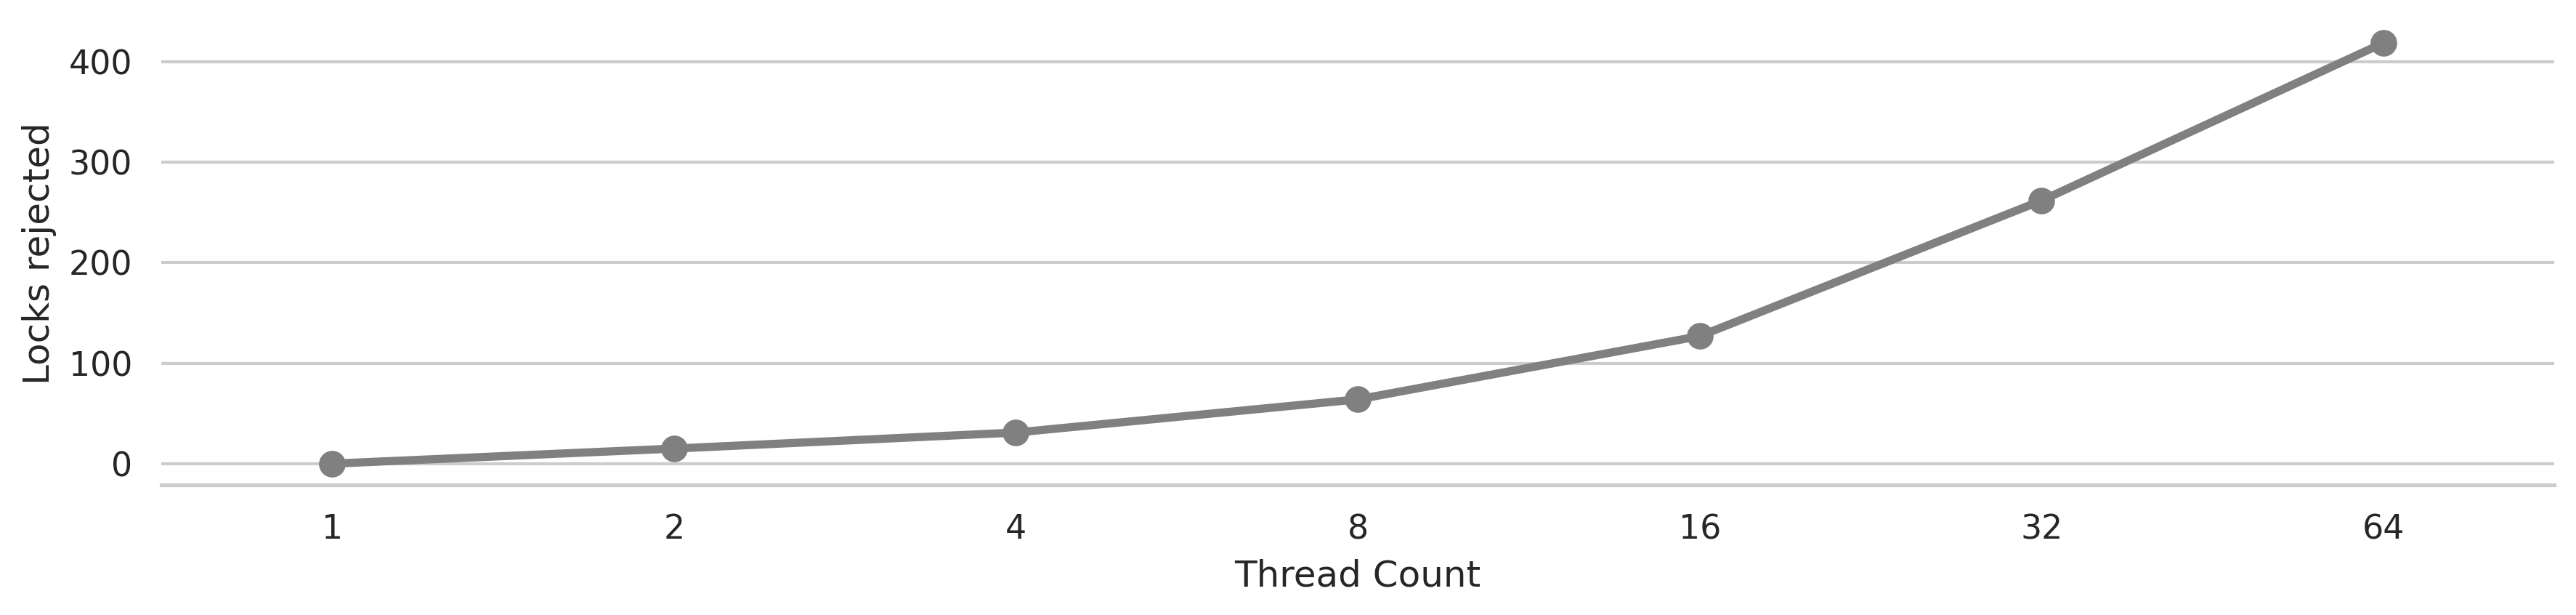
\includegraphics[width=.8\columnwidth]{PerformanceCharts/LockRejection.png}
% % 	\caption{Locks rejected vs Thread Count}
% % 	\label{lockRejection}
% % \end{figure}

% MGL techniques like DomLock, MID, FlexiGran and CALock are slower than coarse and medium grained locks. They are slow for reads and writes due to the presence of false subsumptions between grains causing spurious thread blocks. For structural modifications, DomLock, MID and FlexiGran spend time relabelling the hierarchy which is very expensive. 

% CALock is faster than DomLock, MID and FlexiGran for reads and writes since it avoids false subsumptions (see Section \ref{benchmark:falseSubsumption}). For structual modifications, unlike DomLock, MID and FlexiGran, the relabelling can be parallelised if the lock grains do not overlap. When deleting vertices from the hierarchy (SM1), CALock does not require relabelling. 

% \begin{table*}
% 	\begin{tabular}{l|l|l|l|l|l|l}
% 		\textbf{Operation}	& \textbf{Coarse} 	& \textbf{Medium} 	& \textbf{DomLock} 	&\textbf{MID} 		& \textbf{FlexiGran} 	& \textbf{CALock} \\ \hline
% 		Q1 		& 35 		& 11 		& 560		& 1 		& 589 			& 3 	\\
% 		Q2 		& 43 		& 11 		& 1092 		& 3564 		& 1125 			& 11 	\\
% 		OP6 	& 32 		& 6 		& 560 		& 1 		& 6 			& 4 	\\
% 		OP7 	& 21 		& 1 		& 553 		& 1 		& 7 			& 5 	\\
% 		OP9	 	& 34 		& 3 		& 1 		& 1 		& 3 			& 3 	\\
% 		OP10 	& 31 		& 11 		& 1092 		& 1229 		& 1092 			& 15 	\\
% 		SM2 	& 1 		& 6 		& 556 		& 2427 		& 592 			& 2 	\\
% 		SM3 	& 1 		& 1 		& 560 		& 1266 		& 590 			& 7 	\\

% 	\end{tabular}
% \end{table*}



\section{Metadata management: preprocessing and relabelling} \label
{benchmark:labellingAndRelabelling}
 
MGL techniques rely on metadata to identify lock grains. DomLock and MID use integer intervals for subsumption testing, FlexiGran combines intervals with a level number. CALock, on the other hand, utilizes sets of vertex identifiers. Regardless of the metadata type, excessive housekeeping to maintain its accuracy can easily negate any performance benefits. In this section, we examine the time required to compute the metadata initially (preprocessing) and the time needed to update it after a structural modification (relabeling). The benchmark is run on three different sizes of the STMBench7 graph. Table \ref{tab:graphSizes} lists the size of the STMBench7 hierarchies.

\begin{table}[h]
	\centering
	\captionsetup{justification=centering}
	\begin{tabular}{c|ll}
		\textbf{Graph Size} & \textbf{Vertices} & \textbf{Edges} \\ \hline
		Small  & 234,737 	& 4,393,682 	\\
		Medium & 2,334,257 	& 43,759,682	\\
		Large  & 23,329,457 & 437,419,682 	\\
	\end{tabular}
	\caption{Sizes of the STMBench7 hierarchies}
	\label{tab:graphSizes}
\end{table}


% MGL techniques require metadata to identify the lock grains. DomLock and MID use integer intervals to test subsumption and FlexiGran uses intervals along with a level number. CALock uses sets of vertex identifiers. For any metadata, if the amount of housekeeping required to keep it up to date is high, it can easily negate any achieved performance gains. In this section, we study how long it takes to compute the metadata for the first time (Bulk labelling) and how long it takes to update the metadata after a structural modification (Relabelling).

\subsection{Preprocessing}
We measure the preprocessing time, i.e., the time it takes to assign the labels to a graph for label based MGL techniques like DomLock, MID, FlexiGran and CALock.
This simulates loading data into a database.
This time is measured for three different sizes of the STMBench7 graph. 
The results are shown in Figure \ref{initialLabelling}. 
We observe that DomLock is the fastest since a single depth-first-traversal is sufficient to compute the intervals. MID is 8 times slower than DomLock because it needs to compute two pairs of intervals for each vertex. One computed by a depth-first traversal and another by a depth-first traversal on the mirror image of the graph. FlexiGran is faster than MID but slightly slower than DomLock because of the additional level information that needs to be computed per vertex. 

CALock takes the longest to preprocess a hierarchy since the labels are defined by a recursive breadth-first traversal with a fix-point dependent on the number of paths to a vertex from the root. CALock remains 10 times slower than MID and 20 times slower than DomLock for pre-processing. 

\begin{figure}
	\centering
	\captionsetup{justification=centering}
	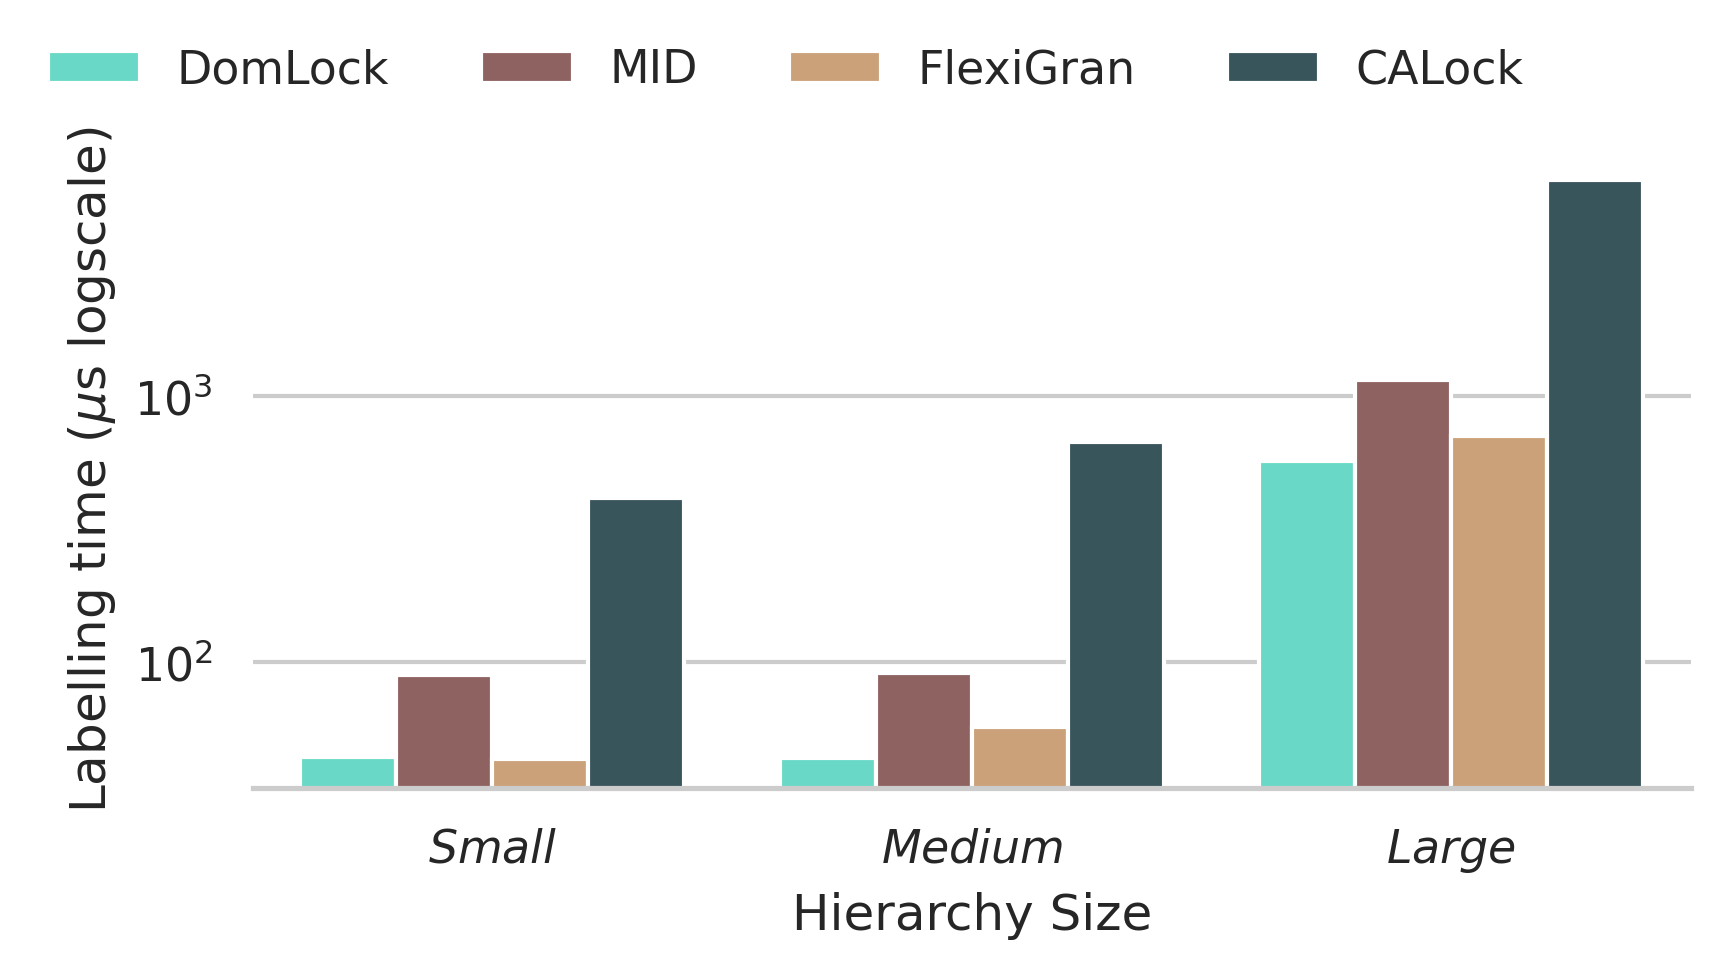
\includegraphics[width=.7\columnwidth]{figures/PerformanceCharts/InitialLabelling}
	\caption{Time to compute initial labels (lower is better)}
	\label{initialLabelling}
\end{figure}


\subsection{Relabelling}
Figure \ref{relabellingTime} shows the average time spent relabelling the graph per structural modification. Coarse grain, medium grain locks and intention locks do not have additional metadata and hence do not require relabelling. 
DomLock, MID and FlexiGran are significantly slow since they relabel the entire graph after a structural modification. This relabelling prevents any concurrent operations. Figure \ref{relabellingTime} shows time taken by DomLock, MID, FlexiGran and CALock to relabel the graph after a structural modification.

% This is because in DomLock, MID and FlexiGran a structural modification anywhere in the graph changes the



% depth-first traversal order of several vertices of the graph. 
% A change in this traversal order requires re-computing a lot of intervals which propagate to the root of the hierarchy. 
% Since the root is involved in the relabeling, intervals are computed under a mutex on the graph which prevents parallel relabelling of disjoint subgraphs leading to poor performance.

In contrast, CALock relabels only the subgraphs directly affected by the structural modification under the same lock as the structural modification.
Thus, multiple grains can be locked, modified and relabelled in parallel. CALock is 100 times faster at relabelling than DomLock, MID and FlexiGran.

%Both DomLock and CALock are faster with a higher number of threads because the STMBench graph slowly becomes less dense as a consequence of vertex deletions which in turn reduces the number of vertices that need to be relabelled.


%\todo{Change figure 9 With the updated results after the run is complete on grid5000}
\begin{figure}[ht]
	\captionsetup{justification=centering}
	\centering
	% \begin{subfigure}[b]{.325\textwidth}
		% \includegraphics[width=\columnwidth]{PerformanceCharts/ReadWithModificationsRelabelling}
		% \caption{R:90\%,W:9.9\%,SM:0.1\%}
	% \end{subfigure}
	% \begin{subfigure}[b]{.32\textwidth}
	% 	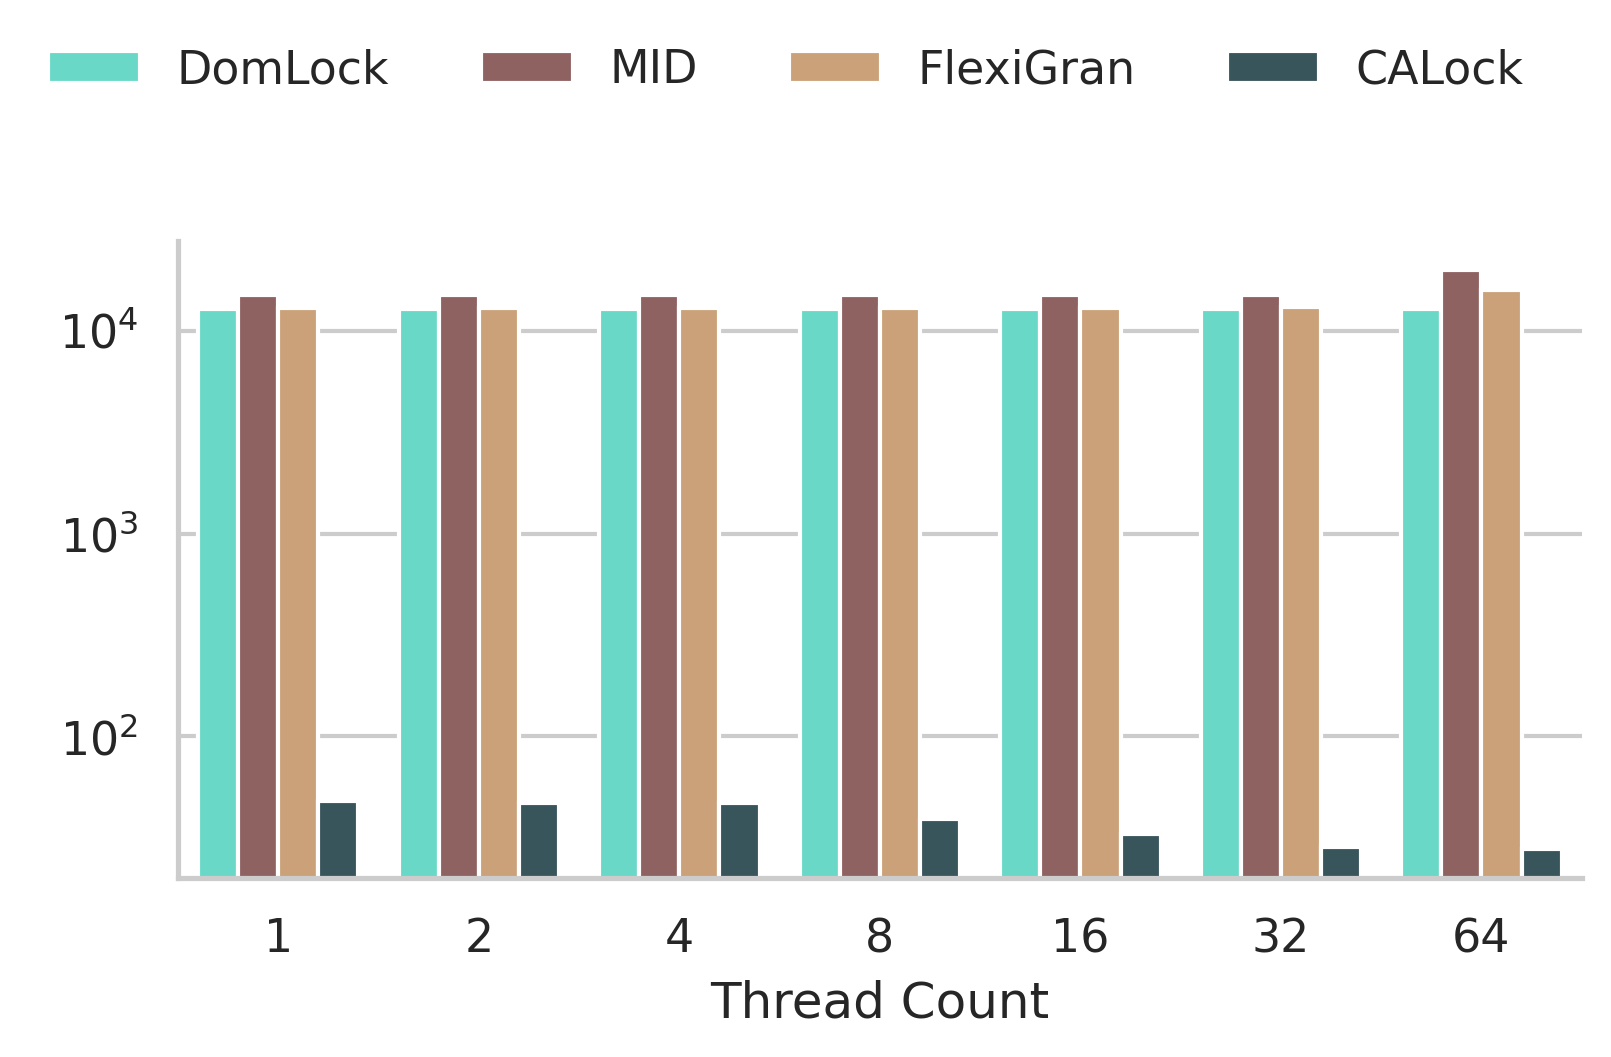
\includegraphics[width=\columnwidth]{PerformanceCharts/BalancedWithModificationsRelabelling}
	% 	\caption{R:60\%,W:39.6\%,SM:0.4\%}
	% \end{subfigure}
	% \begin{subfigure}[b]{.32\textwidth}
		\includegraphics[width=.7\columnwidth]{figures/PerformanceCharts/ReadWithModificationsRelabelling}
	% 	\caption{R:10\%,W:89.1\%,SM:0.9\%}
	% \end{subfigure}
	\caption{Time spent relabelling the graph per structural modification (lower is better)}
	\label{relabellingTime}
\end{figure}

%\todo{Make another benchmark to graph the relabelling time for different types of vertices similar to the subsumption benchmark in figure \ref{nodesLockedPerNodeType}}

\section{Size in memory} \label{benchmark:metadatasize}


Label based MGL techniques utilize metadata to identify the lock grains.
DomLock utilizes integer ranges as labels, which are compact. 
MID uses two pairs of integer ranges to represent the intervals of the vertices.
FlexiGran uses the DomLock intervals along with an integer to store the level of a vertex.
In contrast, CALock employs sets of vertex identifiers as labels, leading to a larger memory footprint.

\begin{figure}[h]
	\centering
	\captionsetup{justification=centering}
	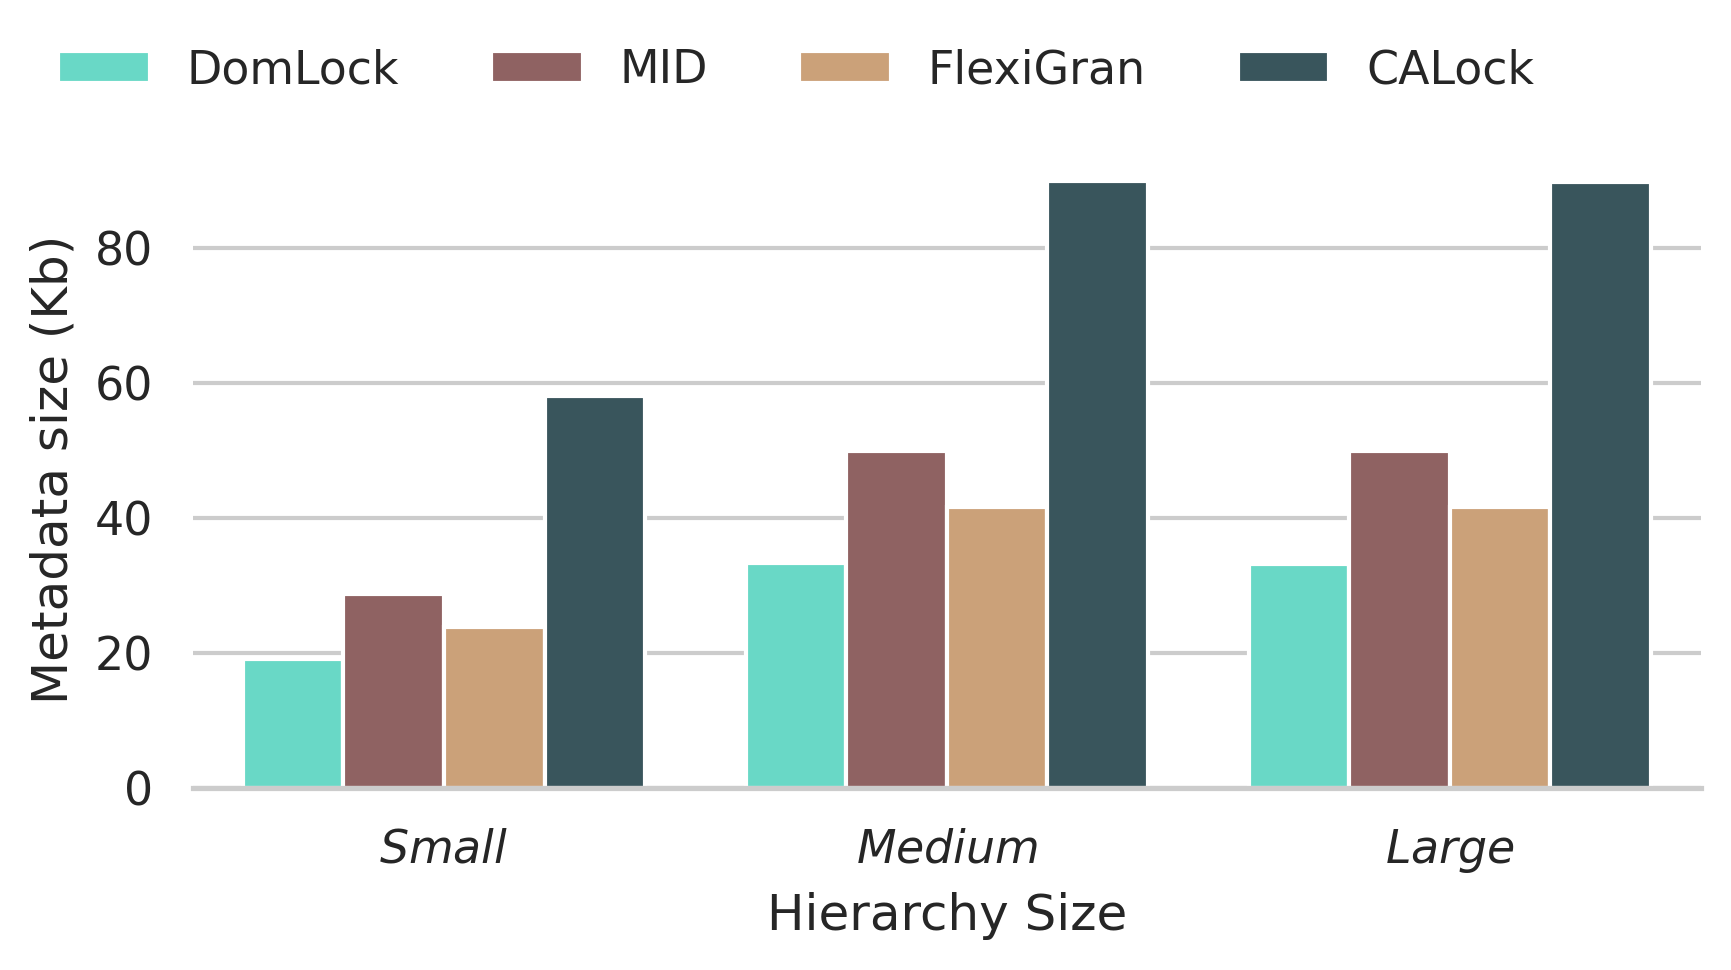
\includegraphics[width=.7\columnwidth]{figures/PerformanceCharts/LabelsMemorySize.png}
 	\caption{Size of the metadata used for labelling in STMBench (lower is better)}
	\label{metadataSize}
\end{figure}

As shown in Figure \ref{metadataSize}, CALock's metadata consumes approximately 1.5$\times$ more memory than DomLock, MID and FlexiGran.
In DomLock, MID and FlexiGran, regardless of the topology of the graph, the label at each vertex consists of integers.
This has low memory requirement however, the information about the exact topology of the hierarchy cannot be inferred from the labelling itself, leading to false subsumptions.
CALock labels, being sets, contain more information allowing for smaller grain sizes and avoid false subsumptions.



\section{Lock granularity and false subsumptions}\label{benchmark:falseSubsumption}

Locking a vertex in MGL implicitly also locks all other vertices present in the lock grain. This allows threads to use a single guard for multiple targets such that the guard is the root of the smallest sub-graph containing the targets. A smaller grain size allows more parallelism and reduces the probability of conflicts. 

To compare the grain sizes for different locking protocols, we measure the number of targets implicitly locked for a guard vertex in the STMBench7 graph. 
Figure \ref{nodesLockedPerNodeType} compares the granularity of DomLock, MID, FlexiGran and CALock.

\begin{figure}[h]
	\centering
	\captionsetup{justification=centering}
	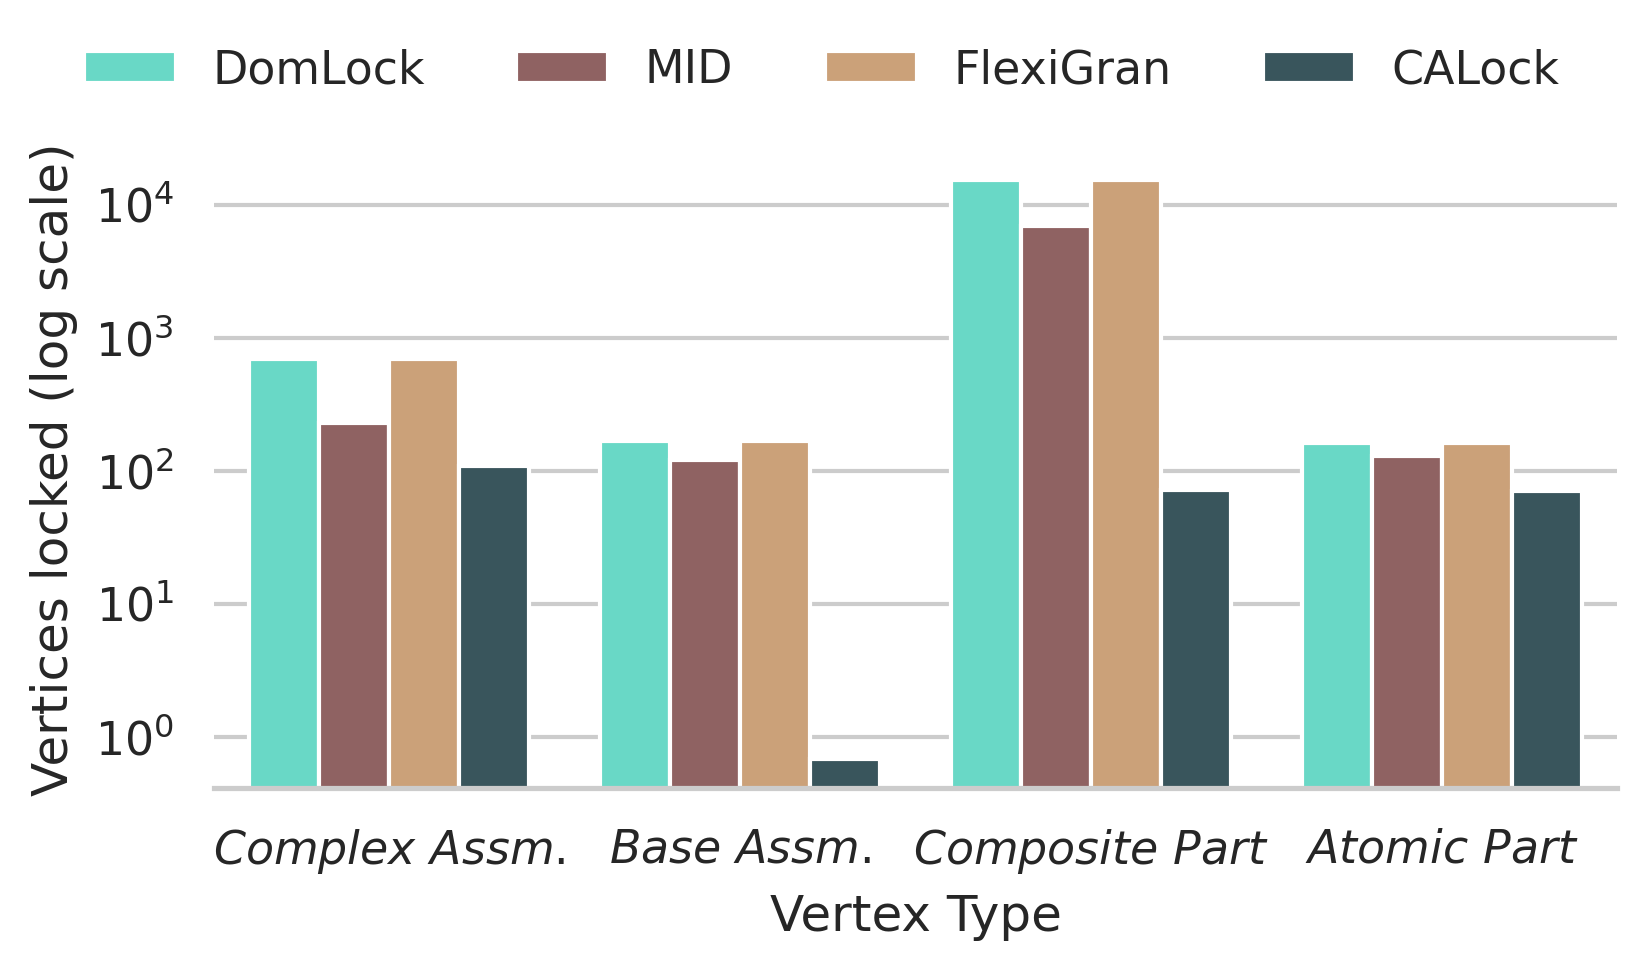
\includegraphics[width=.7\columnwidth]{figures/PerformanceCharts/ContainmentRatio}
	\caption{Vertices locked per vertex type (lower is better)}
	\label{nodesLockedPerNodeType}
\end{figure}

Locking an atomic part has almost the same effect with all algorithms with CALock marginally reducing grain sizes. 
When locking higher up in the graph, the effects vary. 
Locking a complex assembly is more expensive with DomLock, MID and FlexiGran because complex assemblies often share composite parts. Using a complex assembly as a lock guard causes all shared composite parts to be locked leading to large grains. With DomLock, MID and FlexiGran, the grain size is larger 8 times bigger than CALock due to false subsumptions. 

When locking base assemblies, with DomLock, MID and FlexiGran, multiple base assemblies are locked due to the one-to-many relationship between base assemblies and composite parts, again, owing to false subsumptions. CALock is significantly better at this level with grain sizes being 100 times smaller than DomLock, MID and FlexiGran.

Composite parts exhibit a similar trend to base assemblies. CALock has a grain size 100 times smaller than DomLock, MID and FlexiGran. When a composite part is a lock target, the guard is often a base assembly or a complex assembly because a composite part is often contained in multiple base assemblies. This, combined with false subsumptions, leads to large grain sizes for DomLock, MID and FlexiGran.

The granularity of the lock and its effect on subsumption is highly dependent on the topology of the graph. 
False subsumptions aggravate the problem of large grains and lead to more grain overlaps between threads. 
The grain sizes of CALock are always smaller other locking techniques as is evident in Figure \ref{nodesLockedPerNodeType}.


% \subsection{Effect of the lock request size} \label{benchmark:lockRequestSize}
% To study the effect of the size of a lock request on execution time, we set the synthetic benchmark to run a single thread that tries to lock consecutive leaf nodes. 
% A lock request with fewer vertices requires fewer set intersections to identify the LGCA for CALock and fewer integer comparisons to identify the lock interval for DomLock. 
% Figure \ref{requestSize} shows the results.

% \begin{figure}
% 	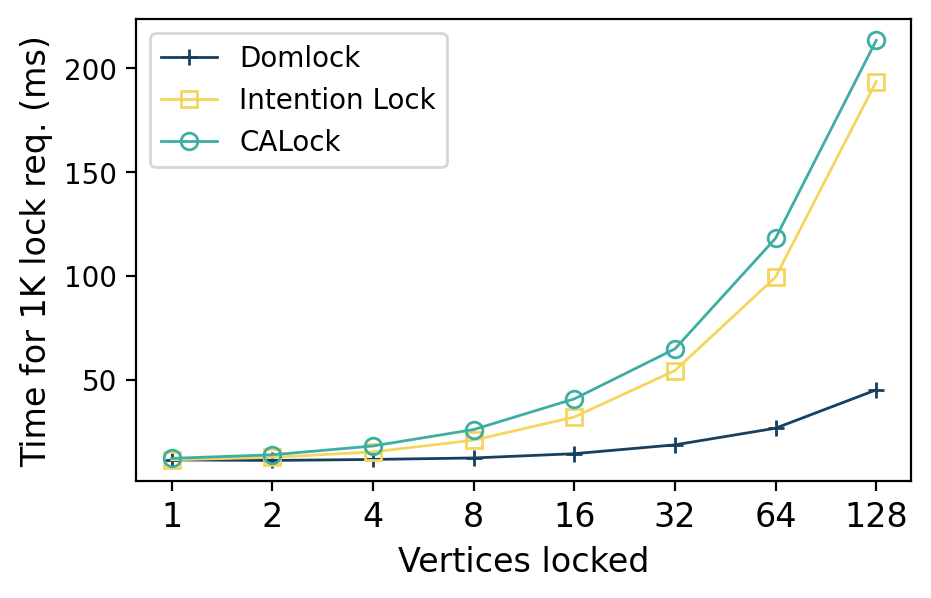
\includegraphics[width=.8\columnwidth]{PerformanceCharts/NodesPerLockRequestTree}
% 	\caption{Effect of lock request size (lower is better)}
% 	\label{requestSize}
% \end{figure}

% For small lock request sizes, the performance of Intention locks, DomLock and CALock is comparable. 
% Their performance diverges as the size of the request increases and DomLock performs best while CALock performs poorly. 
% Intention locks perform better than CALock because the paths to the lock guards are precomputed and stored as an index. 
% This eliminates the need for finding the guard vertex in the graph. 
% Trees have only one path to a vertex which reduces the the cost of placing intention tags along it. 
% The total cost of placing intention tags along the path is linear in the number of vertices being locked.
% %\todo{Complete this section with the details of how in graphs, CALock is better. Also run skewness benchmarks for Graphs. }

% The performance of CALock is poor when accessing several nodes because identifying the position of the lock in the graph requires a set intersection which has higher complexity compared to the integer comparison required for grain identification in DomLock. 
% This is especially bad for trees since the size of the label set for a vertex is equal to the depth of the vertex.


% \subsection{Effect of lock locality} \label{benchmar:lockLocality}

% \begin{figure}
% 	\includegraphics[width=.8\columnwidth]{PerformanceCharts/Skewness}
% 	\caption{Effect of lock locality (lower is better)}
% 	\label{skewedAccess}
% \end{figure}

% To study the effect of the access pattern of the vertices on performance, we configure the stress benchmark to run a fixed number of threads but restrict each thread to access a specific part of the tree for locking. 
% To achieve this, the leaf vertices of the tree are divided into disjoint buckets. A thread picks a bucket at random and creates a lock request for the vertices in that bucket.

% Figure \ref{skewedAccess} shows how this locality affects performance. 
% We observe that when the threads are allowed to lock anywhere in the graph i.e. the bucket size is 1, the probability of conflicts is higher. 
% Due to a large number of conflicts, threads wait longer for their locks and the overall performance degrades. 
% As the locality of access increases and threads are restricted to buckets, the number of conflicts decreases.
% This allows threads to make progress in parallel and leads to higher overall performance. 

\section{Overall locking performance}
Sections \ref{benchmark:PerOpLatency}, \ref{benchmark:labellingAndRelabelling}, \ref{benchmark:metadatasize} and \ref{benchmark:falseSubsumption} studied individual parameters in isolation. Here, we study them together and evaluate their effects on overall performance. 
% For FlexiGran, the percentage of fine-grain locks is set to 50\% as recommended by the authors in their paper \cite{FlexiGran2024}. 
In these set of benchmarks, we study both data updates and structural modifications. 
Figures \ref{staticPerf} and \ref{dynamicPerf} show the throughput of different workloads on static graphs and dynamic graphs respectively. 
The charts in these figures are plotted with the number of concurrent threads on the x-axis and the throughput (op/s) or response time ($\mu s$) on the y-axis. 
Response time is measured from when the thread issues a lock request until the lock is granted.


\subsection{Data Accesses} \label{benchmark:StaticOverallPerf}

% \begin{figure*}
% 	\centering
% 	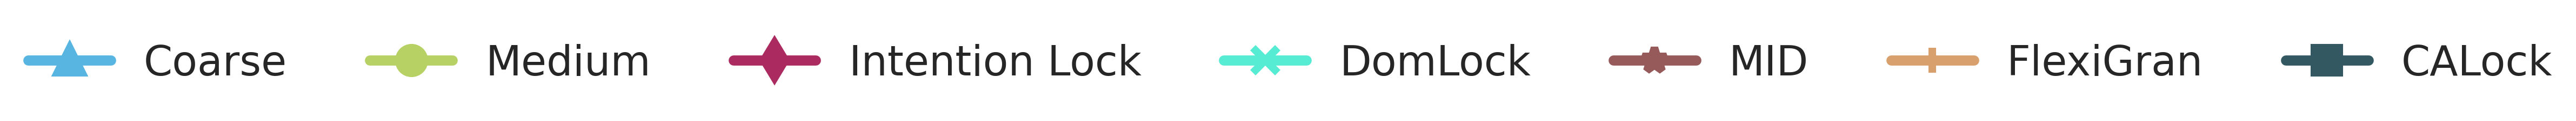
\includegraphics[width=.9\textwidth]{figures/PerformanceCharts/Legend}
% \end{figure*}

\begin{figure*}[ht]
	\centering
	\captionsetup{justification=centering}
	\begin{subfigure}[b]{\textwidth}
		\centering
		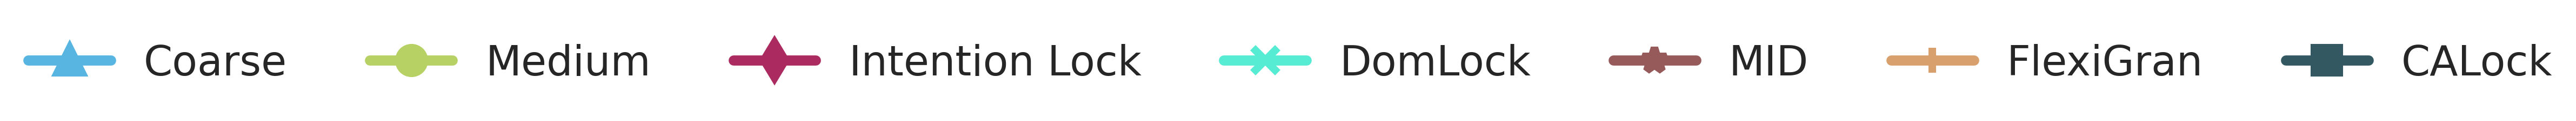
\includegraphics[width=\textwidth]{figures/PerformanceCharts/Legend}
	\end{subfigure}
	\begin{subfigure}{.33\textwidth}
		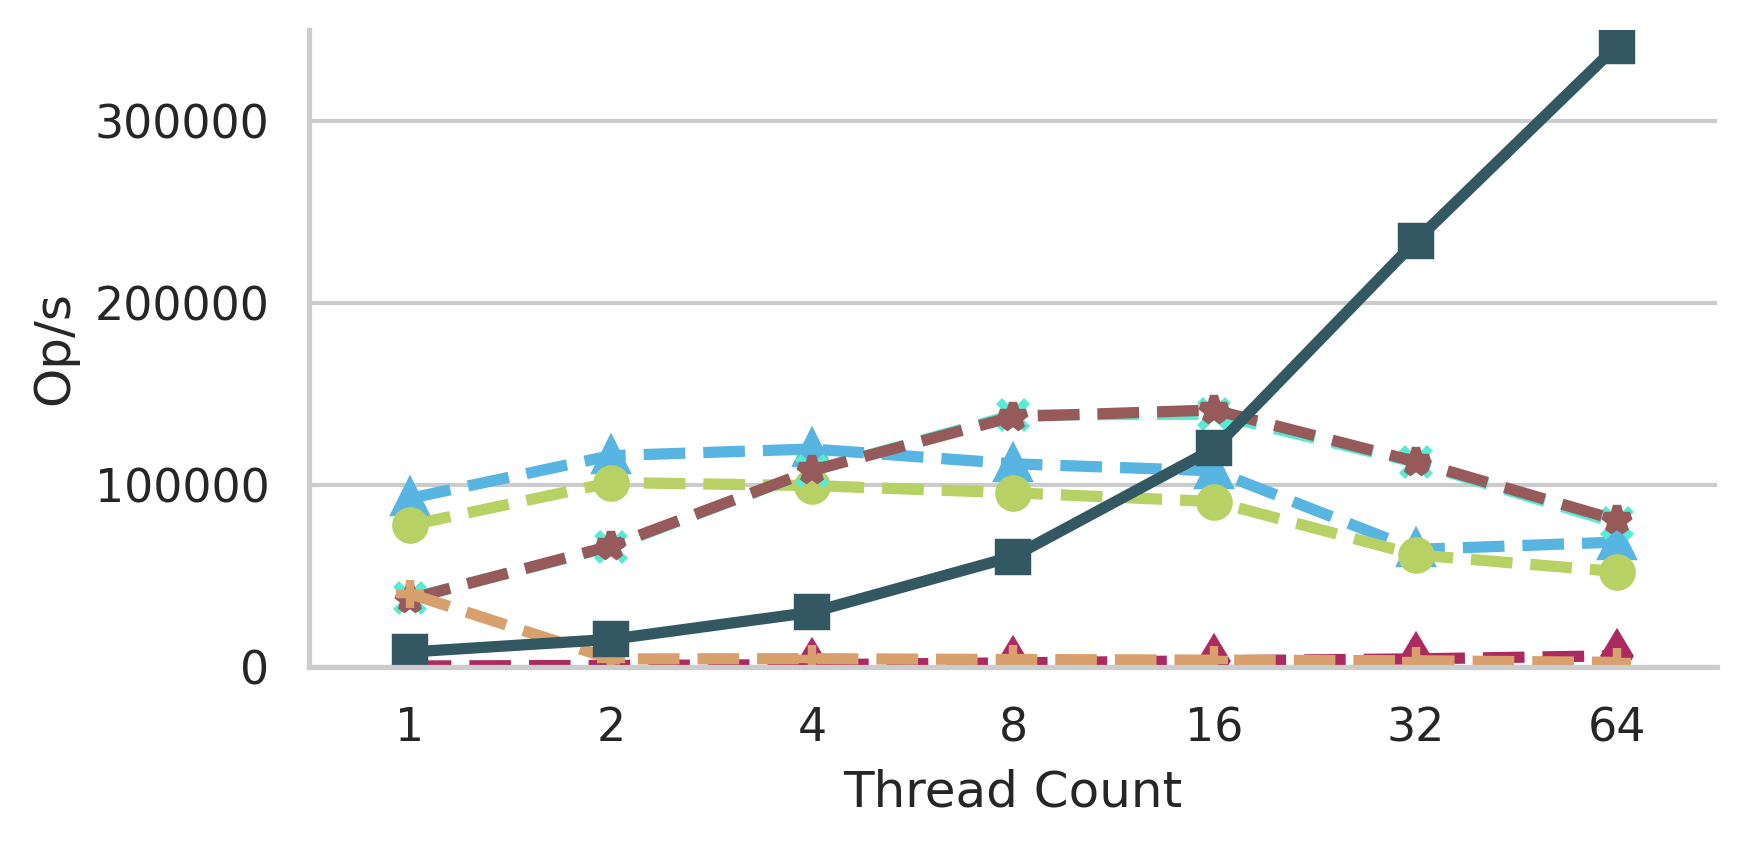
\includegraphics[width=\textwidth]{figures/PerformanceCharts/ReadWithoutModificationsThroughput}
		\caption{R:90\%,W:10\%}
		\label{rwm}
	\end{subfigure}
	\begin{subfigure}{.32\textwidth}
		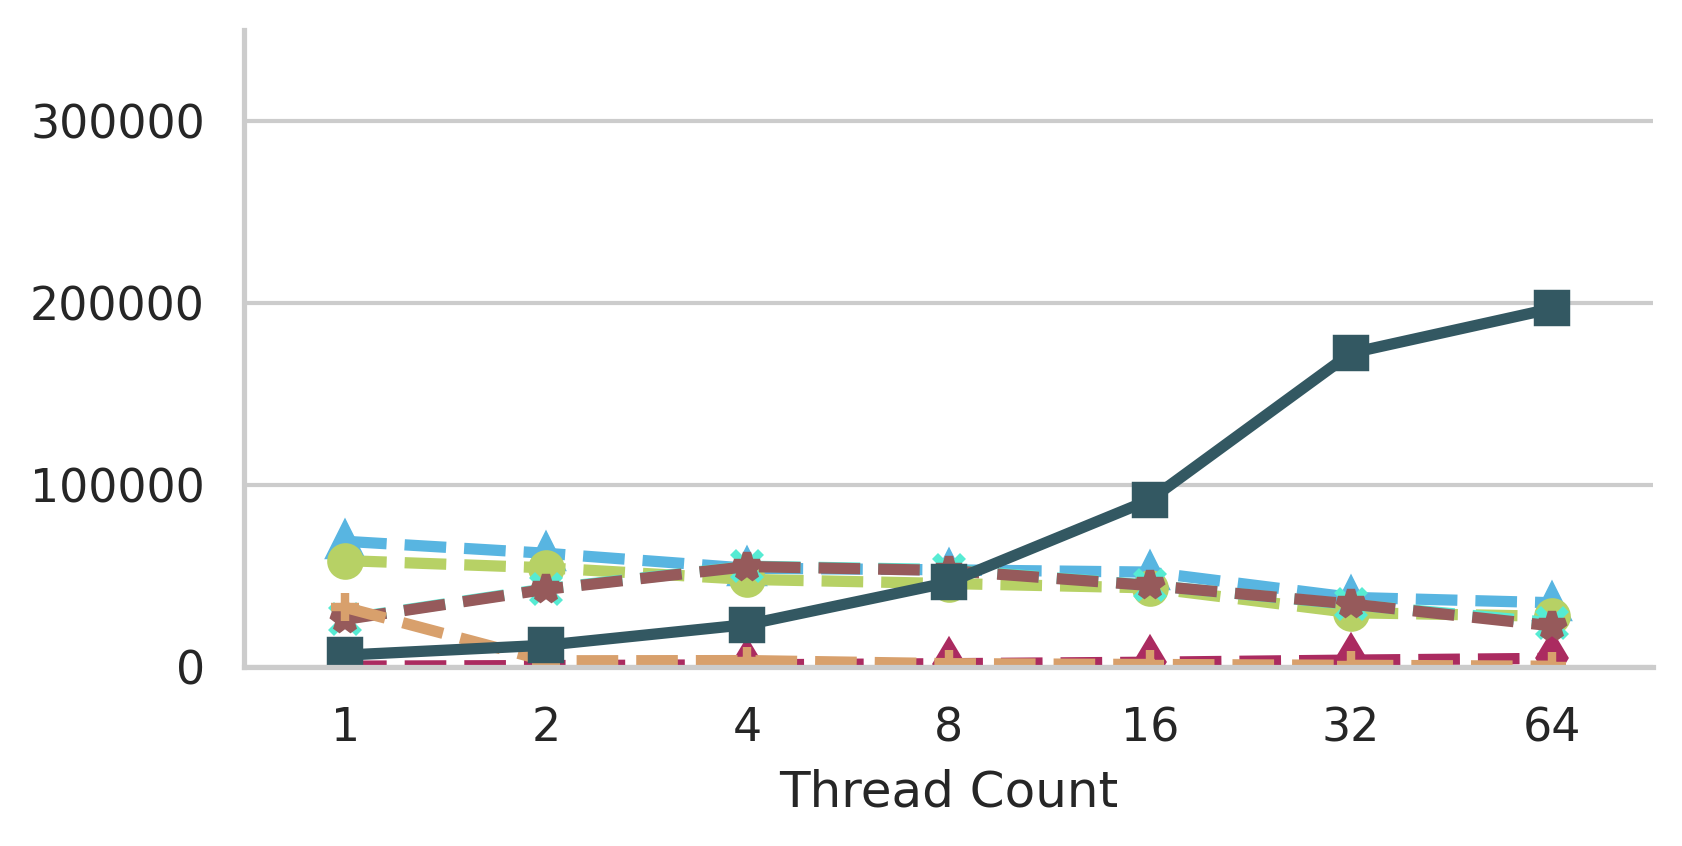
\includegraphics[width=\textwidth]{figures/PerformanceCharts/BalancedWithoutModificationsThroughput}
		\caption{R:60\%,W:40\%}
		\label{bwm}
	\end{subfigure}
	\begin{subfigure}{.32\textwidth}
		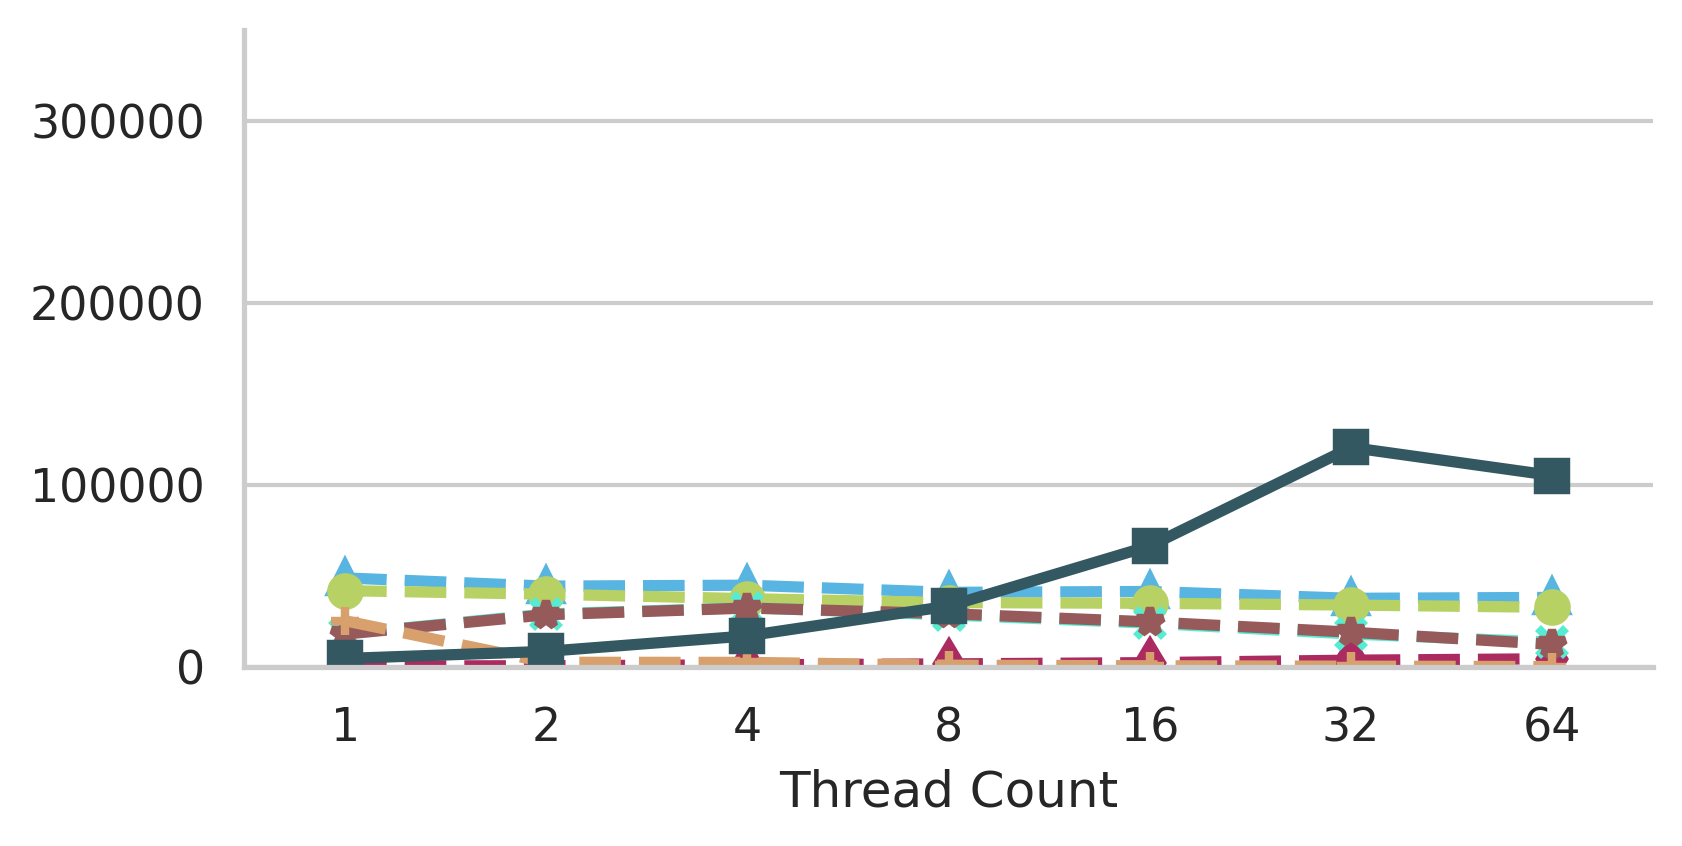
\includegraphics[width=\textwidth]{figures/PerformanceCharts/WriteWithoutModificationsThroughput}
		\caption{R:10\%,W:90\%}
		\label{wwm}
	\end{subfigure}
	\begin{subfigure}[b]{\textwidth}
		\caption*{\ref{rwm}, \ref{bwm}, \ref{wwm}: Throughput (higher is better)}
	\end{subfigure}


	\begin{subfigure}[b]{.33\textwidth}
		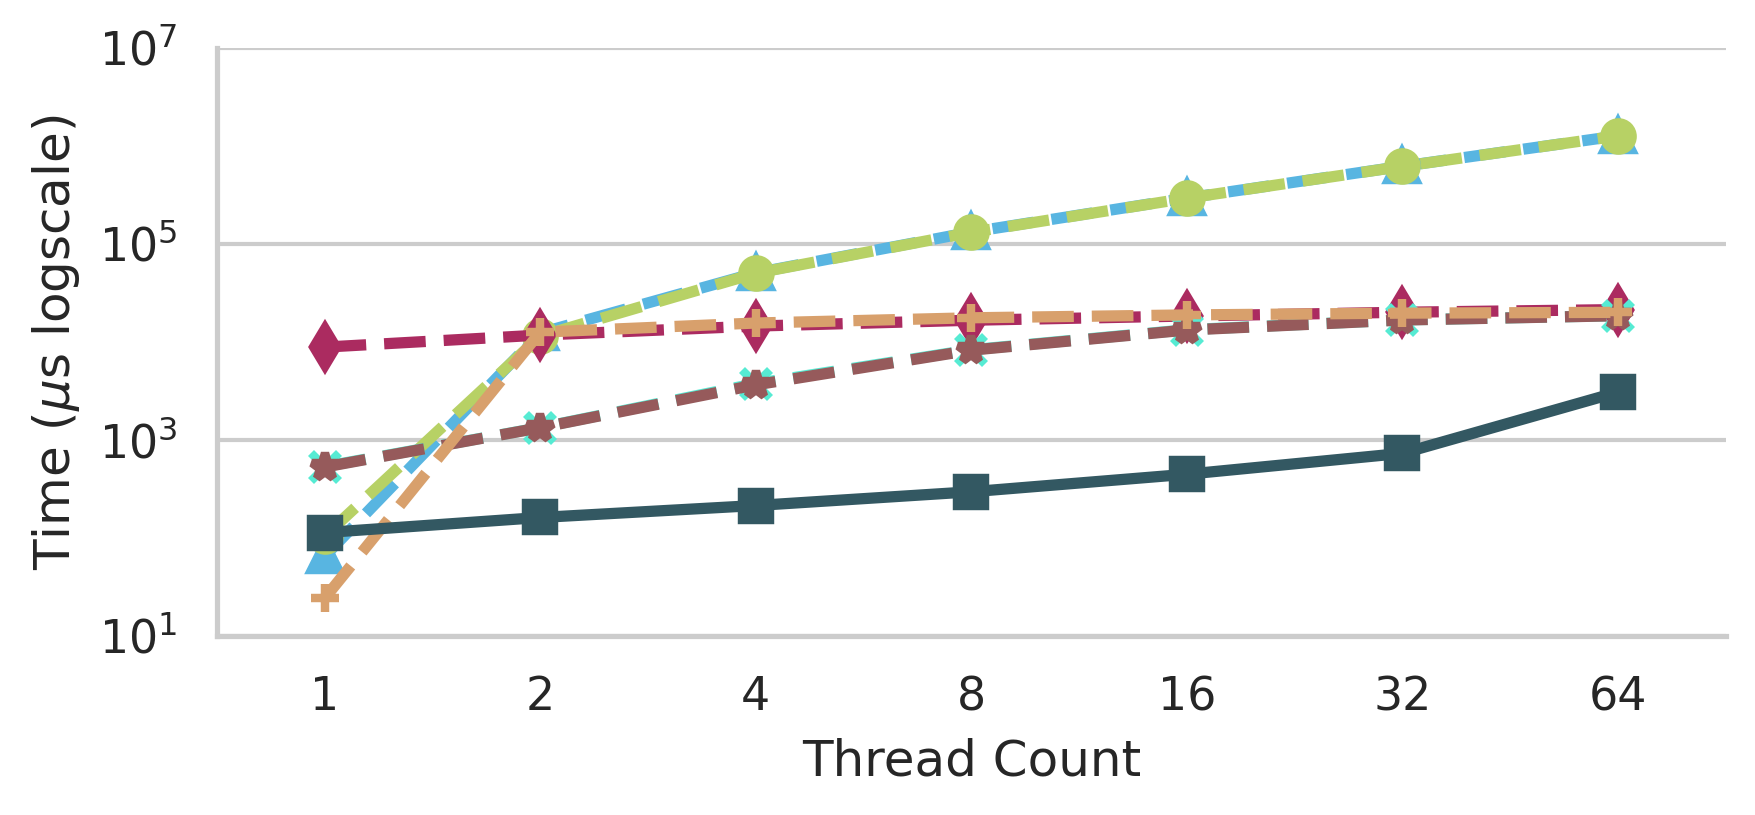
\includegraphics[width=\textwidth]{figures/PerformanceCharts/ReadWithoutModificationsIdleness}
		\caption{R:90\%,W:10\%}
		\label{irwm}
	\end{subfigure}
	\begin{subfigure}[b]{.32\textwidth}
		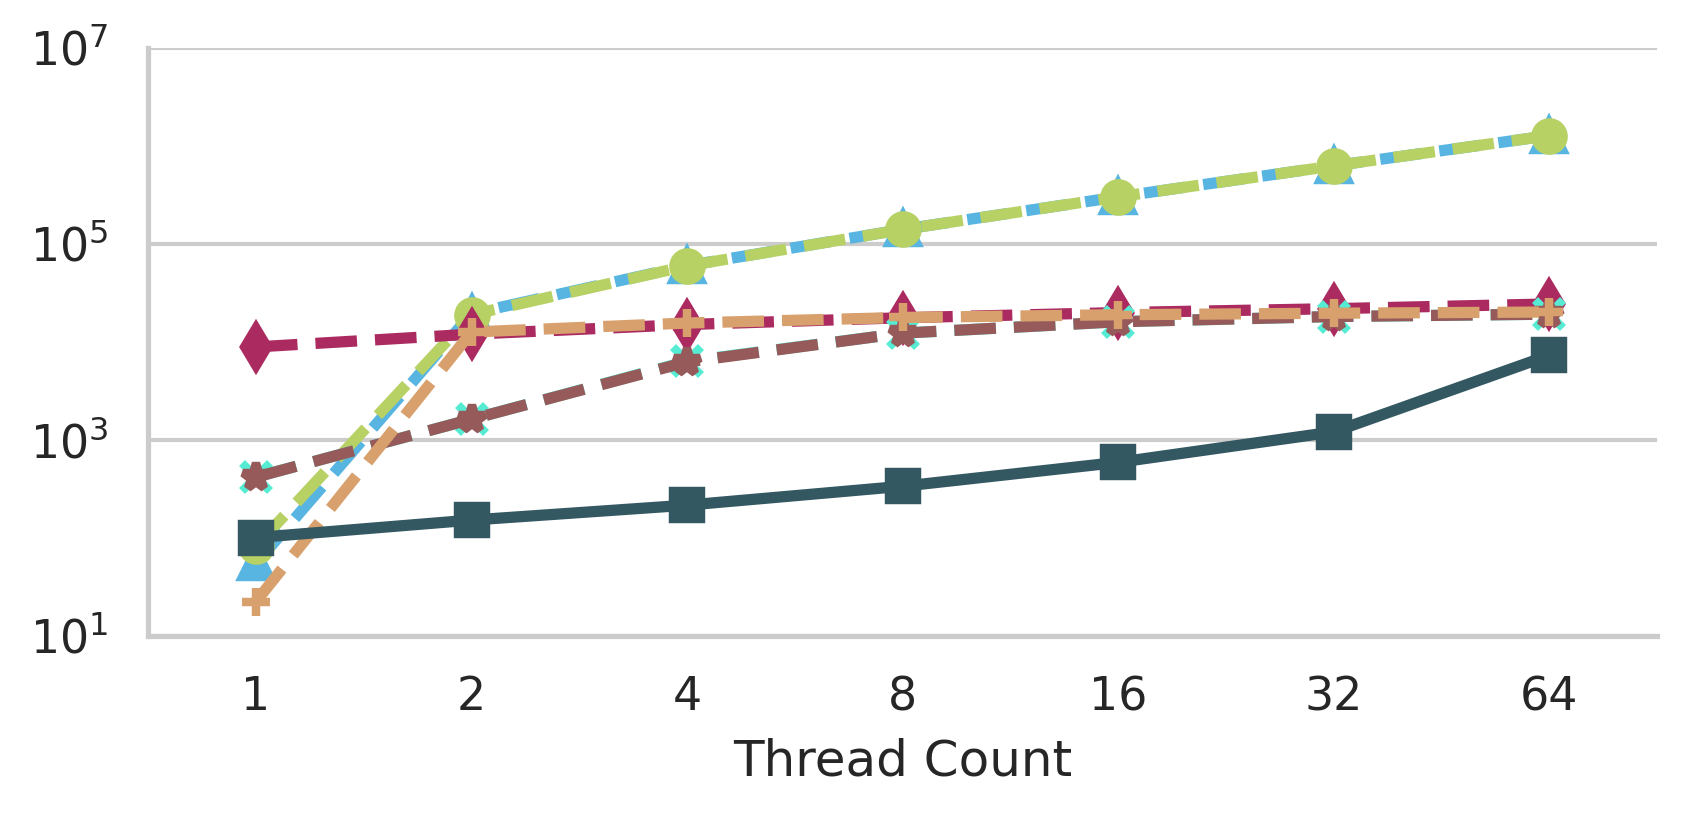
\includegraphics[width=\textwidth]{figures/PerformanceCharts/BalancedWithoutModificationsIdleness}
		\caption{R:60\%,W:40\%}
		\label{ibwm}
	\end{subfigure}
	\begin{subfigure}[b]{.32\textwidth}
		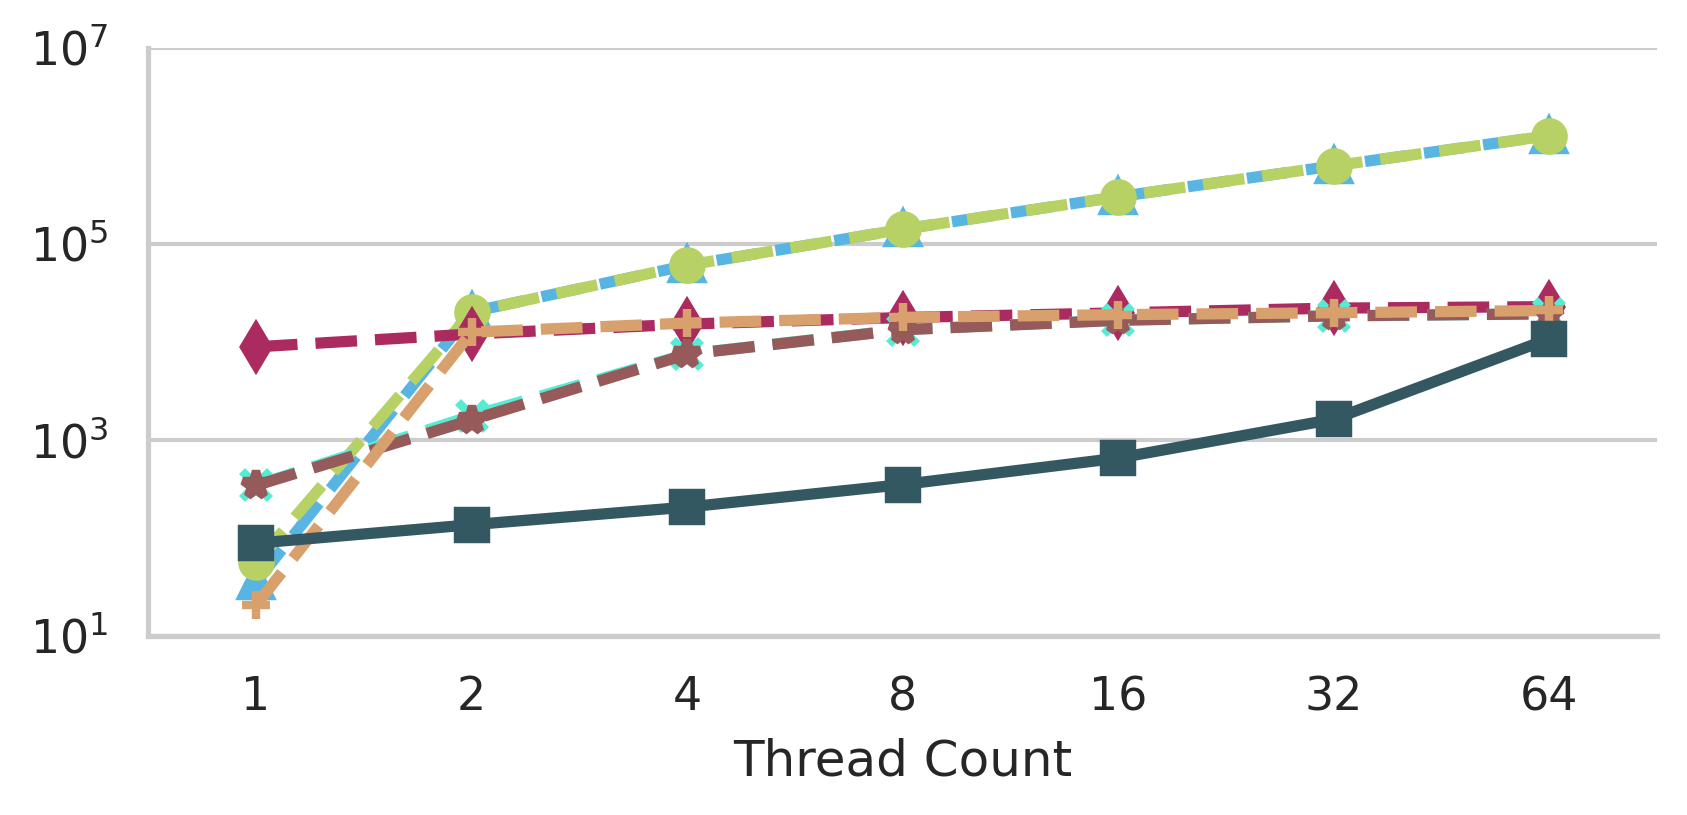
\includegraphics[width=\textwidth]{figures/PerformanceCharts/WriteWithoutModificationsIdleness}
		\caption{R:10\%,W:90\%}
		\label{iwwm}
	\end{subfigure}
	\begin{subfigure}[b]{\textwidth}
		\caption*{\ref{irwm}, \ref{ibwm}, \ref{iwwm}: Average time to grant lock request (lower is better)}
	\end{subfigure}



	\caption{Performance with different workload types on static graphs (R: reads, W: writes).}
	\label{staticPerf}
	\end{figure*}
Throughput figures \ref{rwm}, \ref{bwm} and \ref{wwm} show that coarse-grain and medium-grain locks have better throughput for up to 4 concurrent threads due to the additional computation of the lock grain required for DomLock, MID, FlexiGran and CALock. Beyond 4 threads, MGL techniques give better throughput. However, the performance of DomLock and MID stagnates at 8 threads.

The graph in STMBench is irregular and has multiple paths leading to a vertex. DomLock, MID and Flexigran intervals often lead to false subsumptions (see Section \ref{benchmark:falseSubsumption}). Intention locks exhibit poor performance due to the high number of paths leading to target vertices from the root of the STMBench hierarchy (see Section\ref{ttc}).

CALock successfully minimizes the size of the lock grains and allows threads to lock disjoint grains in parallel, achieving better scalability than DomLock, MID and FlexiGran.
We observe that CALock is at least 2 times faster than DomLock for 32 threads and at least 4.5 times faster than DomLock for 64 threads.

% Observe that as the ratio of writes in a workload increases, the maximum throughput of any locking mechanism decreases because of inherent contention due to conflicts between write lock requests.


% Figure \ref{allReadPercentage} shows the trend of performance gain with an increasing ratio of reads for 32 concurrent readers/writers. 
% We see that as the proportion of reads increases, the performance of CALock and DomLock improves because reads can happen concurrently. However, DomLock is still slower than CALock because of false subsumptions that cause spurious thread blocking.

Response time figures \ref{irwm}, \ref{ibwm} and \ref{iwwm} compare the wait time per thread between coarse-grain locks, medium-grain locks, Intention locks,  DomLock, MID, FlexiGran and CALock.
Response time increases with the number of threads due to an increase in conflicts.
For a single thread, coarse-grain and medium-grain locks are the fastest, but their performance suffers with any form of parallelism. 

Between the MGL techniques, FlexiGran and Intention lock take the longest to grant a lock on average. With Intention locks, this is because of the cost of traversals required to acquire intention locks on vertices. With FlexiGran, lock conflict detection is expensive because of the coexistence of MGL and fine-grain locks. DomLock and MID are faster than FlexiGran but, remain significantly slower than CALock. 

In interval-based MGL techniques like DomLock, MID and FlexiGran, once a lock request identifies an interval it wishes to lock, the thread traverses the hierarchy to find the corresponding lock guard with the requested interval (or. interval pair for MID). This traversal is especially expensive when locking deeper in the hierarchy. CALock on the other hand computes the guard vertex directly by a set intersection, not requiring a traversal giving faster response times for lock requests. 

For all locking protocols, the overall wait time increases with the number of concurrent threads, because of an increase in the number of conflicts due to overlapping grains. For 64 threads, CALock is 6 times faster than DomLock in a read-dominated load and 1.5 times faster in a write-dominated load.



	% \begin{figure}
	% 	\captionsetup{justification=centering}
	% 	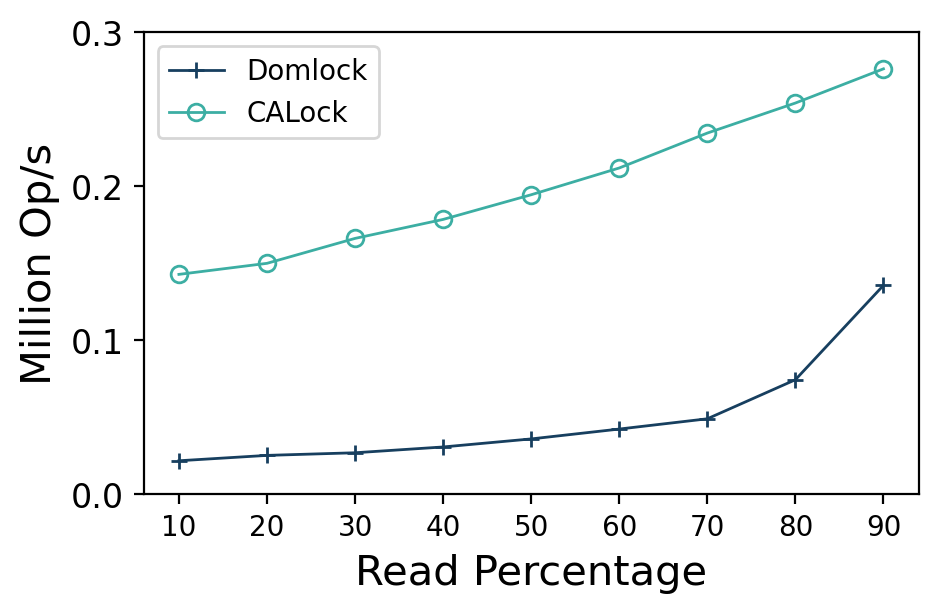
\includegraphics[width=0.8\columnwidth]{PerformanceCharts/ReadPercentageThroughput}
	% 	\caption{Comparing Domlock and CAlock with different read proportions on 32 threads (higher is better)}
	% 	\label{allReadPercentage}
	% \end{figure}


			% for which the improvement is slower but always remains better than DomLock overall.
			%\todo{Change the improves much faster line to something that says domlock is still bad.}


	



\subsection{Structural Modifications} \label{benchmark:DynamicOverallPerf}

A structural modification changes the topology of the graph. This triggers relabelling for MGL locking techniques like DomLock, MID, FlexiGran and CALock. 
% Structural modifications happen under a mutex for coarse grain locks, medium grain locks, DomLock, MID and FlexiGran. 
Throughput figures \ref{rm}, \ref{bm} and \ref{wm} show the performance of locking algorithms when reads and writes interleave with structural modifications.
We set structural modifications to 1\% of the total writes.
For example in Figure \ref{bwm}, 40\% of the operations are writes. Out of these writes, 10\% are structural modifications, i.e. $40\% \times 1\%  = 0.4\%$ structural modifications. The remaining 39.6\% are data writes.


\begin{figure*}[h]
	\centering
	\captionsetup{justification=centering}
		\begin{subfigure}[b]{\textwidth}
			\centering
			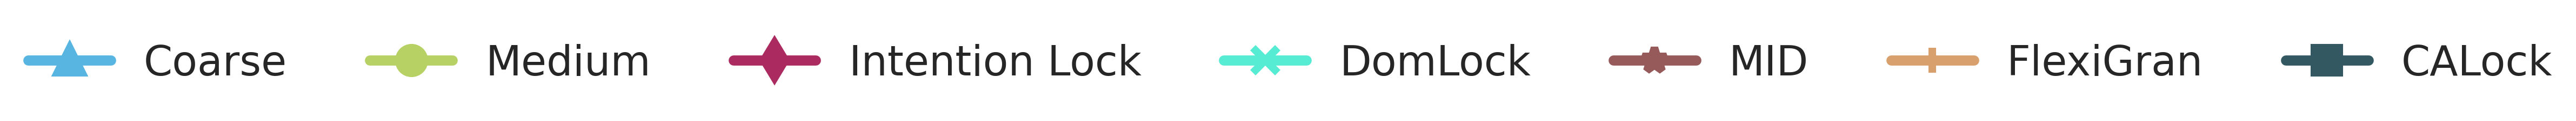
\includegraphics[width=\textwidth]{figures/PerformanceCharts/Legend}
		\end{subfigure}
		\begin{subfigure}[b]{.33\textwidth}
			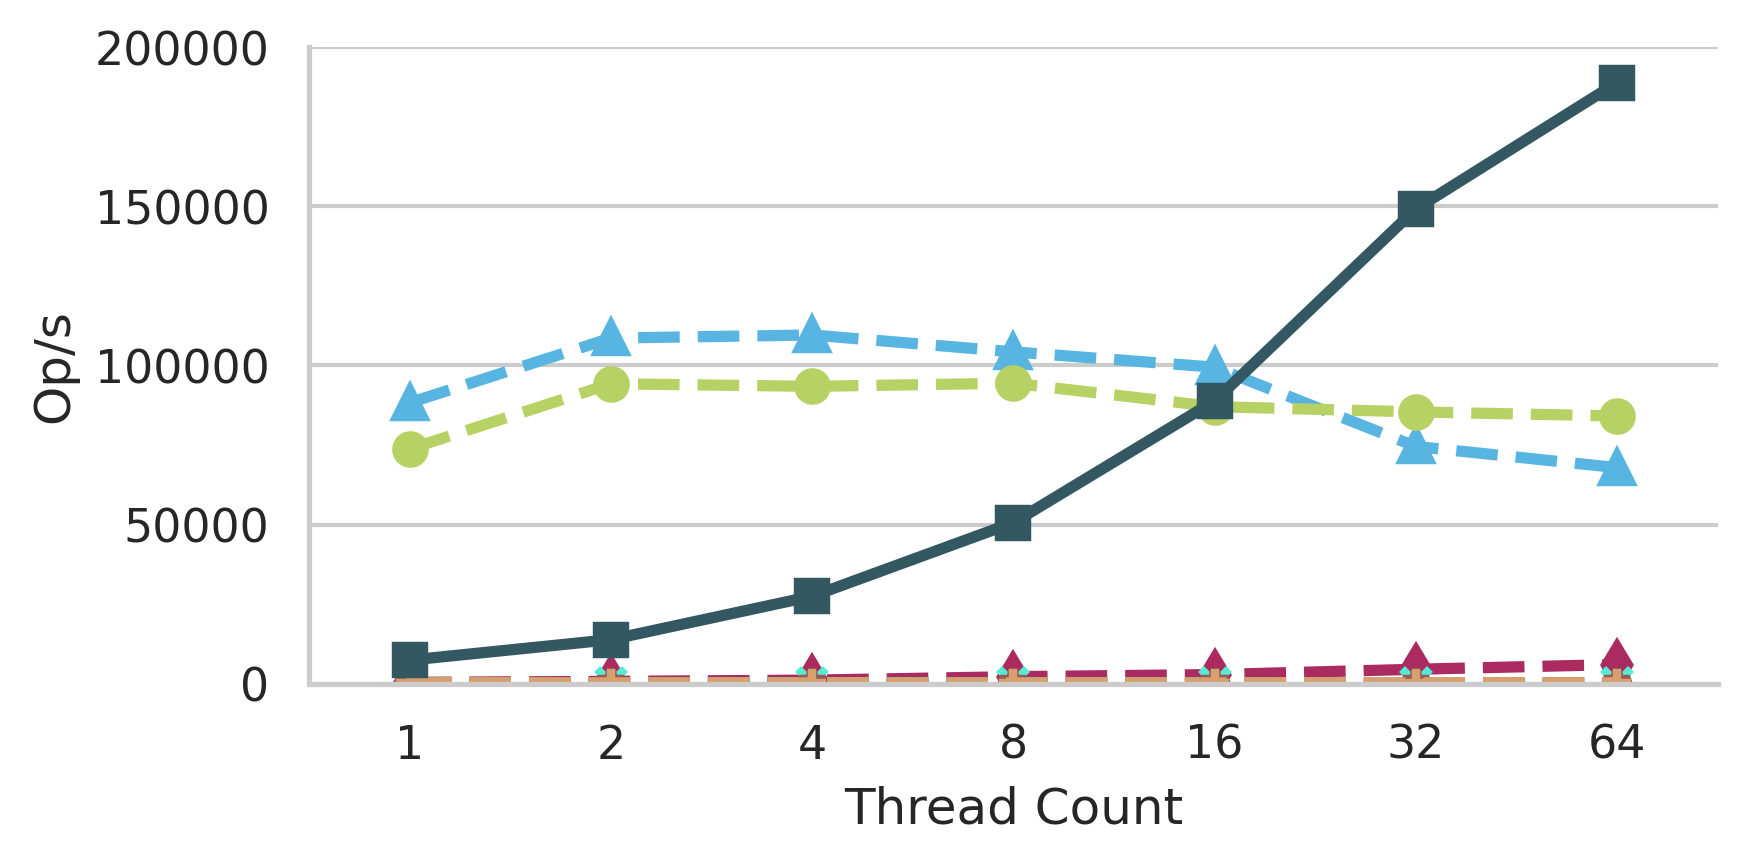
\includegraphics[width=\textwidth]{figures/PerformanceCharts/ReadWithModificationsThroughput}
			\caption{R:90\%,W:9.9\%,SM:0.1\%}
			\label{rm}
		\end{subfigure}
		\begin{subfigure}[b]{.325\textwidth}
			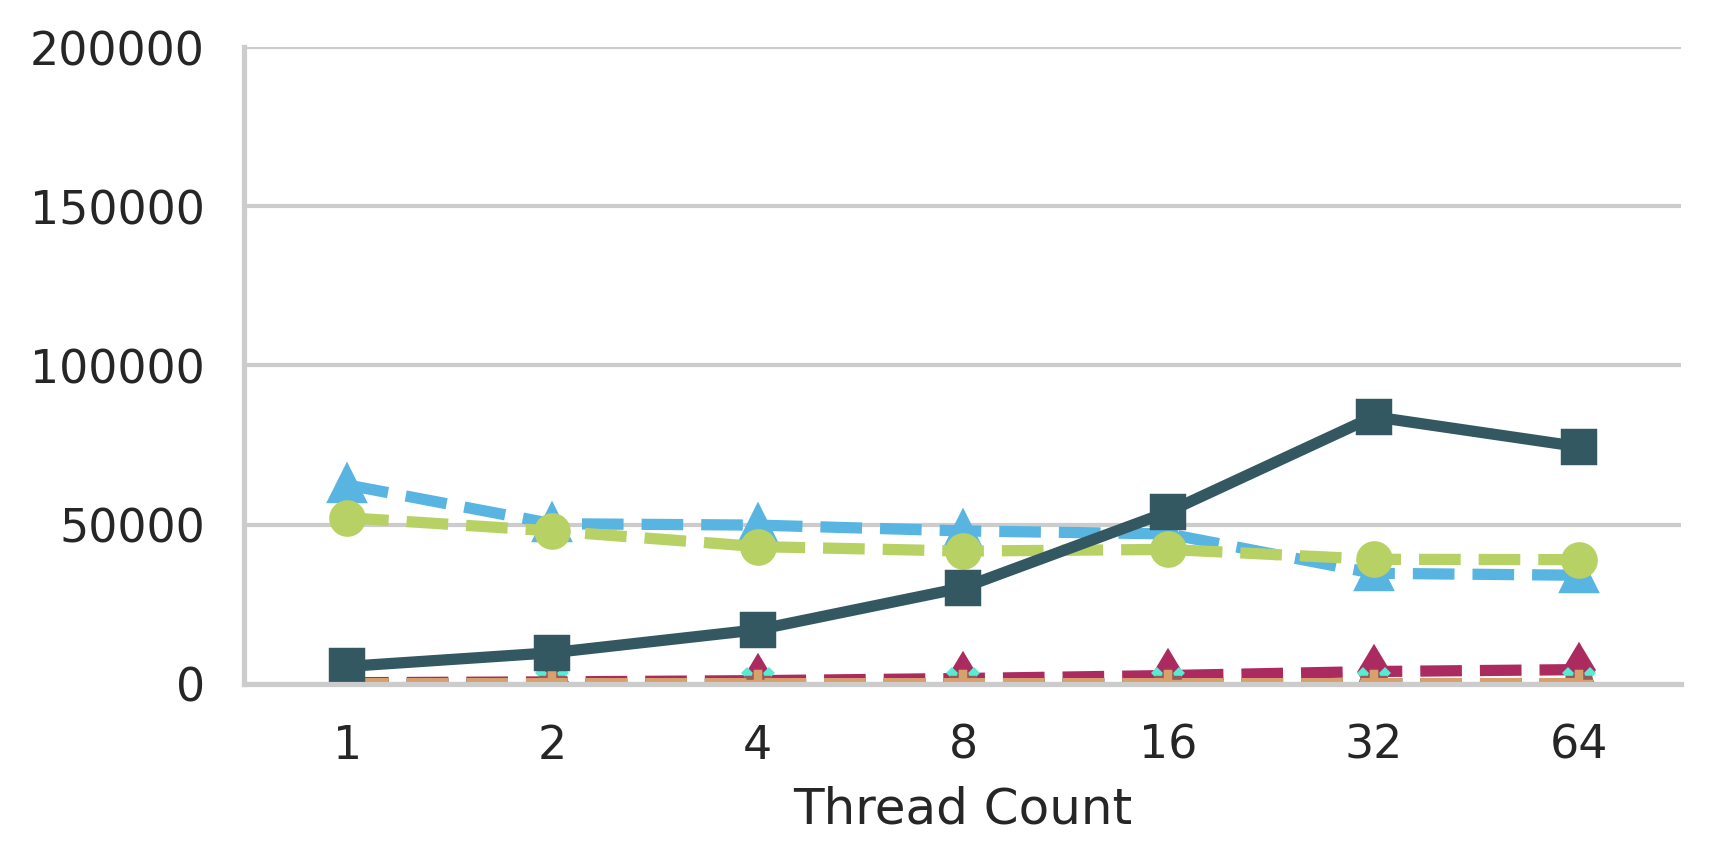
\includegraphics[width=\textwidth]{figures/PerformanceCharts/BalancedWithModificationsThroughput}
			\caption{R:60\%,W:39.6\%,SM:0.4\%}
			\label{bm}
		\end{subfigure}
		\begin{subfigure}[b]{.325\textwidth}
			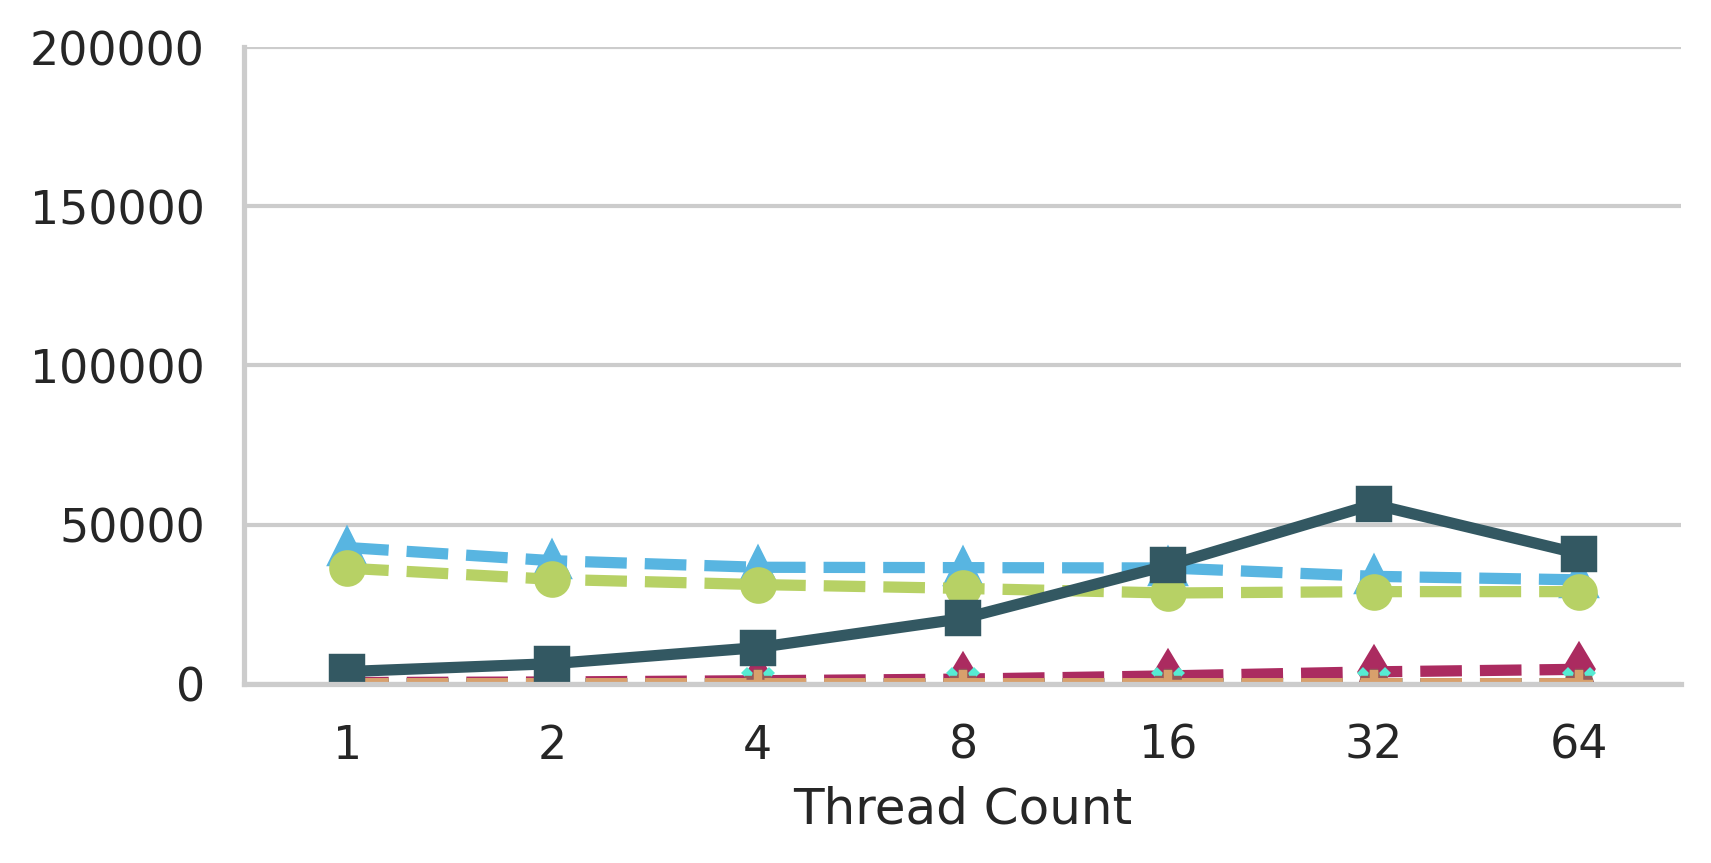
\includegraphics[width=\textwidth]{figures/PerformanceCharts/WriteWithModificationsThroughput}
			\caption{R:10\%,W:89.1\%,SM:0.9\%}
			\label{wm}
		\end{subfigure}
		\begin{subfigure}[b]{\textwidth}
			\caption*{\ref{rm}, \ref{bm}, \ref{wm} : Throughput (higher is better)}
		\end{subfigure}
	
	
	
		\begin{subfigure}[b]{.33\textwidth}
			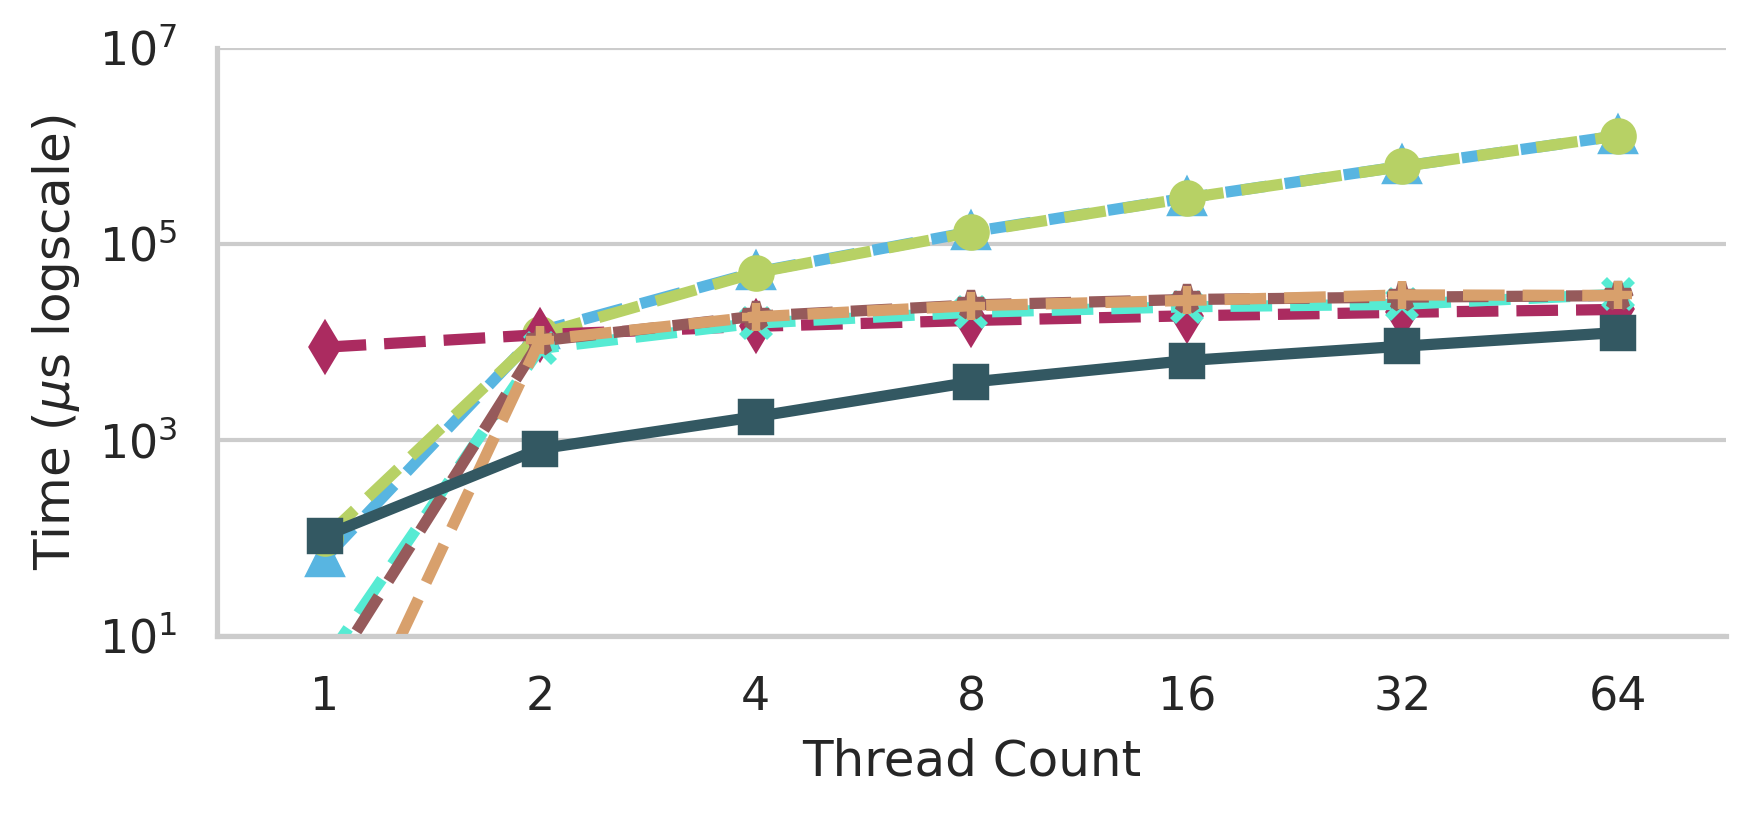
\includegraphics[width=\textwidth]{figures/PerformanceCharts/ReadWithModificationsIdleness}
			\caption{R:90\%,W:9.9,SM:0.1\%}
			\label{irm}
		\end{subfigure}
		\begin{subfigure}[b]{.325\textwidth}
			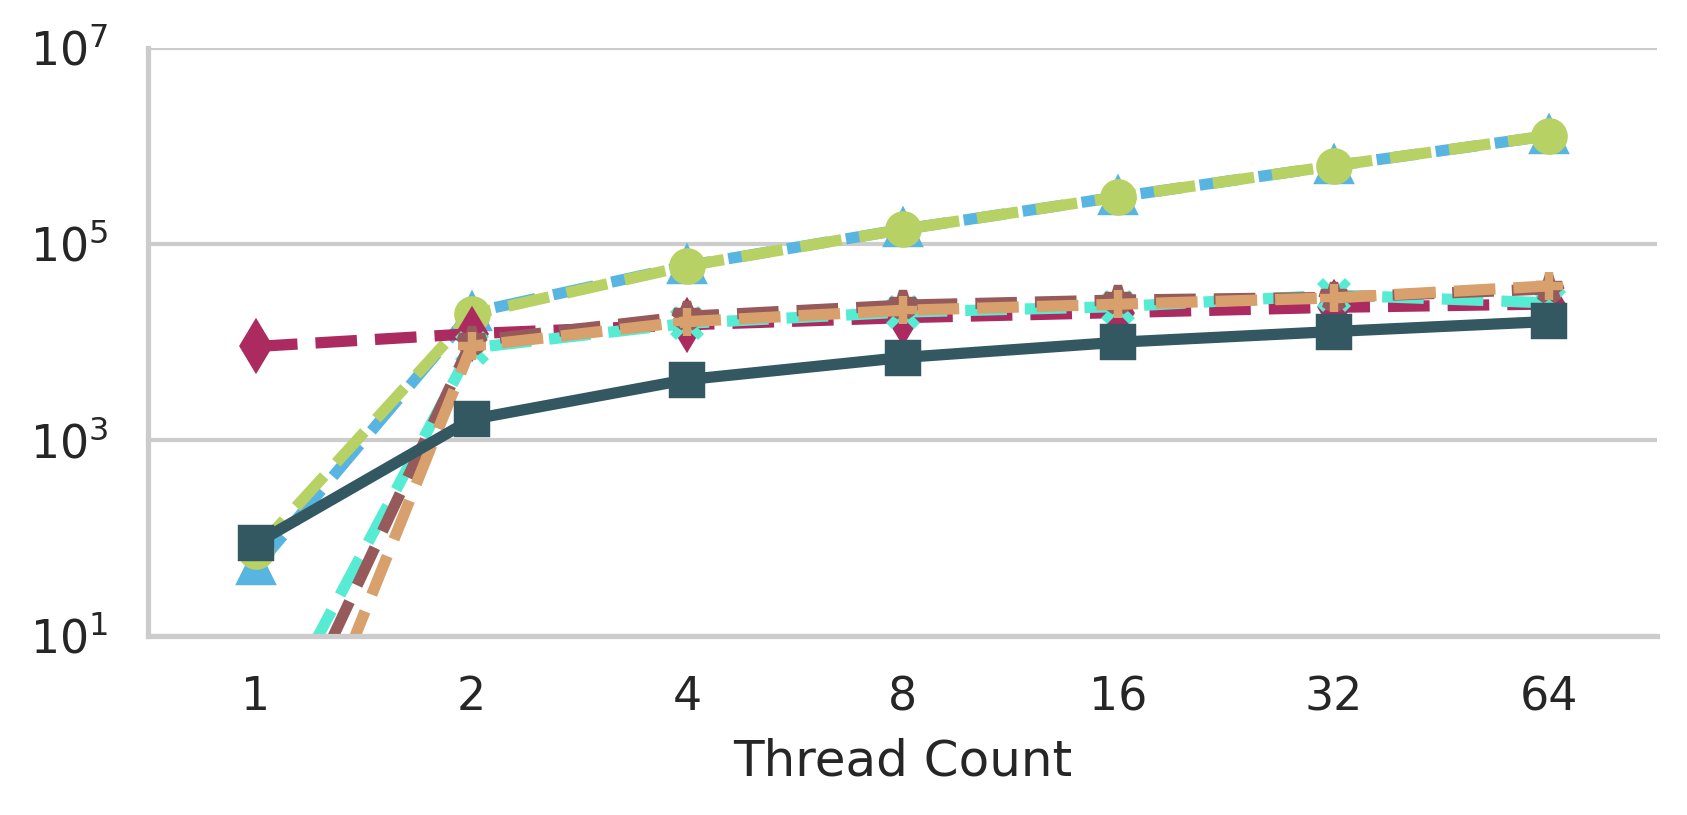
\includegraphics[width=\textwidth]{figures/PerformanceCharts/BalancedWithModificationsIdleness}
			\caption{R:60\%,W:39.6\%,SM:0.4\%}
			\label{ibm}
		\end{subfigure}
		\begin{subfigure}[b]{.325\textwidth}
			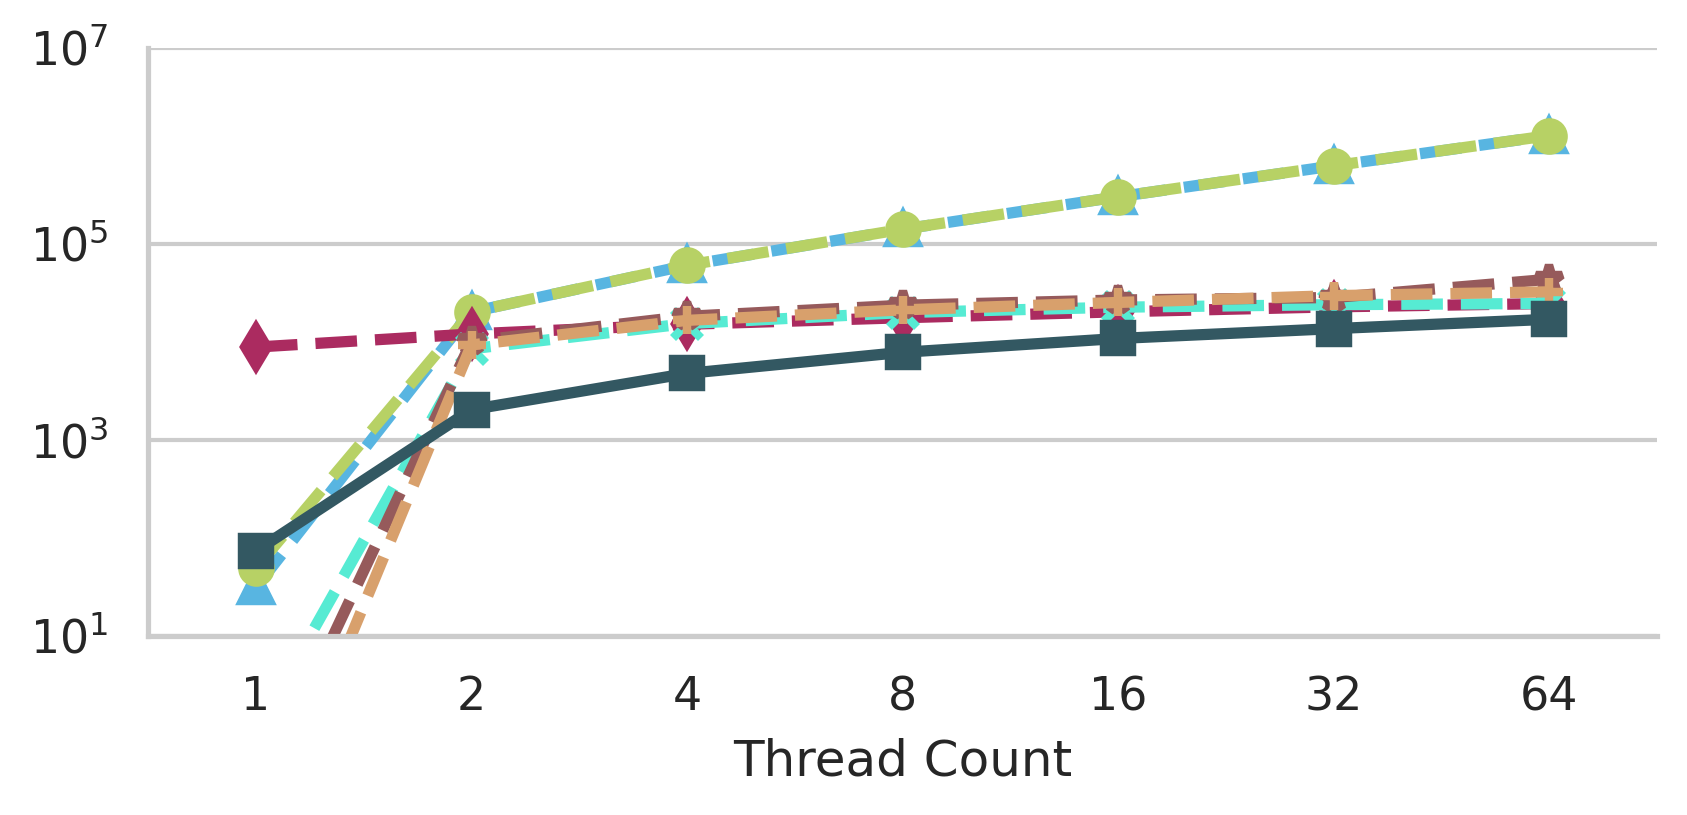
\includegraphics[width=\textwidth]{figures/PerformanceCharts/WriteWithModificationsIdleness}
			\caption{R:10\%,W:89.1\%,SM:0.9\%}
			\label{iwm}
		\end{subfigure}
		\begin{subfigure}[b]{\textwidth}
			\caption*{\ref{irm}, \ref{ibm}, \ref{iwm}: Average time to grant lock request  (lower is better)}
		\end{subfigure}
	
		\caption{Performance with different workload types on dynamic graphs  (R: reads, W: writes; SM: structural modifications).}
		\label{dynamicPerf}
	\end{figure*}

In a write-heavy workload (Throughput figure \ref{wm}), structural modifications can be as high as 0.9\%. 
While in read-heavy workloads (Throughput figure \ref{rm}), they are as low as 0.1\%.
Even under a small fraction of structural modifications, we observe that Intention locks, coarse-grain and medium-grain locks do not scale with the number of threads. 
% Intention locks are no different. While structural modifications do not require any additional care in intention locks, the cost of placing intention tags on a huge number of vertices is proportionally high.

	
DomLock, MID and FlexiGran perform significantly worse compared to other algorithms because along with the lack of parallelism due to an additional relabelling required when a structural modification occurs.
Note that the curves in Throughput figures \ref{rm}, \ref{bm} and \ref{wm} for DomLock, MID and FlexiGran are relatively flat, indicating a lack of scalability. CALock can parallelize structural modifications and is 2x faster than coarse and medium-grained locks and about 8x faster than DomLock, MID and FlexiGran.

Response time for Intention locks remains same regardless of the proportion of structural modifications. However, as shown in Response time figures \ref{irm}, \ref{ibm} and \ref{iwm}, response time for DomLock, MID and FlexiGran is longer for workloads with structural modifications compared to workloads without.
Response time for CALock also increases for dynamic graphs when compared to static graphs but CALock remains faster than all other lock techniques for even the most contended workload.

	%Figures \ref{irm}, \ref{ibm} and \ref{iwm} plot the wait time per thread between DomLock and CALock in the presence of structural modifications. We observe that the wait time for DomLock requests is significantly higher. This is because the structural modification operations in DomLock require a mutex and block every other thread.


\section{Summary of experimental results}
% \subsection{Discussion}
% The initial labelling time is proportional to the size of the graph but in conjunction with other benchmark results, CALock is a better choice for runtime performance since the fast integer labels of DomLock, MID and FlexiGran require more expensive relabelling when the graph is modified by structural modification operations (see Section \ref{benchmark:labellingAndRelabelling}).

% Based on the results of the synthetic benchmarks, Intention locks are a good candidate for regular static graphs and DomLock might still be a better approach compared to CALock if relabelling is not required because the graph is static. However, CALock is a better choice for dynamic graphs since the total relabelling cost is lower (see Section \ref{benchmark:DynamicOverallPerf}).

\subsection{Summary}
With the results from the experiments using STMBench7 and microbenchmarks, we can derive the following conclusions.
\begin{itemize}
	\item Intention locks are the most expensive locking technique for any STMBench workload and are not suitable for irregular graphs.
	\item CALock is faster than DomLock, coarse-grain locks and medium-grain locks for all studied workloads with more than 8 concurrent threads.

	\item In read heavy workloads without structural modifications, CALock is at least 3 times faster compared to any other locking technique.

	\item  In read heavy workloads with structural modifications, CALock is 1.5 times faster than coarse-grain and medium-grain locks and 8x faster than DomLock, MID and FlexiGran.

	\item In write heavy workloads without structural modifications, CALock is 2 times faster than coarse-grained and medium-grained locks and 4 times faster than DomLock, MID and FlexiGran

	\item In write heavy workloads with structural modifications, CALock performs as good as coarse-grain and medium-grain locks and 4 times faster than DomLock, MID and FlexiGran

	\item CALock is an appropriate locking technique if the graph is irregular and the workload consists of structural modifications (for which DomLock, MID and FlexiGran are unsuitable).
\end{itemize}
